%% Le lingue utilizzate, che verranno passate come opzioni al pacchetto babel. Come sempre, l'ultima indicata sar� quella primaria.
%% Se si utilizzano una o pi� lingue diverse da "italian" o "english", leggere le istruzioni in fondo.
\def\thudbabelopt{english,italian}
%% Valori ammessi per target: bach (tesi triennale), mst (tesi magistrale), phd (tesi di dottorato).
\documentclass[target=mst]{thud}[2014/03/11]

%% Aggiunta pacchetto per inserimento di immagini
\usepackage{graphicx}
\usepackage{mathtools}

\usepackage{listings}
\usepackage{color}

\definecolor{codegreen}{rgb}{0,0.6,0}
\definecolor{codegray}{rgb}{0.5,0.5,0.5}
\definecolor{codepurple}{rgb}{0.58,0,0.82}
\definecolor{backcolour}{rgb}{0.95,0.95,0.92}

%% Custom style per i listing
\lstdefinestyle{customcpp}{
        language=C++,
		backgroundcolor=\color{backcolour},   
		commentstyle=\color{codegreen},
		keywordstyle=\color{magenta},
		numberstyle=\tiny\color{codegray},
		stringstyle=\color{codepurple},
		basicstyle=\footnotesize,
		breakatwhitespace=false,         
		breaklines=true,                 
		captionpos=b,                    
		keepspaces=true,                 
		numbers=left,                    
		numbersep=5pt,                  
		showspaces=false,                
		showstringspaces=false,
		showtabs=false,                  
		tabsize=2
}

%% Setting globale per i listing: stile di default customcpp
\lstset{style=customcpp}

\usepackage{capt-of}
\graphicspath{ {img/Introduzione/} {img/ContestoTecnologico/1_PCNEurotech/} {img/ContestoTecnologico/2_TecnTesi/} {img/CorpoTesi/1_AmbientiLavoro/} {img/CorpoTesi/2_PCNBackSub/} }

%% --- Informazioni sulla tesi ---
%% Per tutti i tipi di tesi
\title{Elaborazione di Immagini in ambito Embedded con OpenCV: Passenger Counter}
\author{Mattia Dal Ben}
\course{Ingegneria Elettronica}
\supervisor{Prof.\ Antonio Abramo}
\cosupervisor{Ing.\ Marco Carrer}
%% Altri campi disponibili: \reviewer, \tutor, \chair, \date (anno accademico, calcolato in automatico).
%% Con \supervisor, \cosupervisor, \reviewer e \tutor si possono indicare pi� nomi separati da \and.
%% Per le sole tesi di dottorato
\phdnumber{313}
\cycle{XXVIII}
\contacts{Via della Sintassi Astratta, 0/1\\65536 Gigatera --- Italia\\+39 0123 456789\\\texttt{http://www.example.com}\\\texttt{inbox@example.com}}
\rights{Tutti i diritti riservati a me stesso e basta.}
%% Campi obbligatori: \title, \author e \course.

%% --- Pacchetti consigliati ---
%% hyperref: Regola le impostazioni della creazione del PDF... pi� tante altre cose.
%% tocbibind: Inserisce nell'indice anche la lista delle figure, la bibliografia, ecc.

%% --- Stili di pagina disponibili (comando \pagestyle) ---
%% sfbig (predefinito): Apertura delle parti e dei capitoli col numero grande; titoli delle parti e dei capitoli e intestazioni di pagina in sans serif.
%% big: Come "sfbig", solo serif.
%% plain: Apertura delle parti e dei capitoli tradizionali di LaTeX; intestazioni di pagina come "big".

\begin{document}

%% Il frontespizio prima di tutto!
\maketitle

%% Dedica (opzionale)
%% \begin{dedication}A mia madre.\end{dedication}

%% Ringraziamenti (opzionali)
%% \acknowledgements
%% Sed vel lorem a arcu faucibus aliquet eu semper tortor. Aliquam dolor lacus, semper vitae ligula sed, blandit iaculis leo. Nam pharetra lobortis leo nec auctor. Pellentesque habitant morbi tristique senectus et netus et malesuada fames ac turpis egestas. Fusce ac risus pulvinar, congue eros non, interdum metus. Mauris tincidunt neque et aliquam imperdiet. Aenean ac tellus id nibh pellentesque pulvinar ut eu lacus. Proin tempor facilisis tortor, et hendrerit purus commodo laoreet. Quisque sed augue id ligula consectetur adipiscing. Vestibulum libero metus, lacinia ac vestibulum eu, varius non arcu. Nam et gravida velit.

%% Sommario (opzionale)
\abstract
Nello sviluppo di questa tesi si \`e affrontato lo studio e la progettazione di un sistema di conteggio dei passeggeri su una piattaforma embedded. Il software applicativo \`e basato su algoritmi di elaborazione di immagine resi disponibili dalla libreria open-source per l'image processing OpenCV. La piattaforma software \`e stata realizzata utilizzando il progetto Yocto, il quale permette la creazione di distribuzioni Linux customizzate e targettate all'utilizzo in abito embedded.
L'applicazione di Passenger Counter ha come scopo quello di contare i passeggeri che attraversano in entrata e in uscita le porte di un mezzo pubblico, in modo tale da permettere un conteggio esatto delle persone presenti sul mezzo.
Lo sviluppo si \`e diviso in quattro fasi principali:
\begin{itemize}
\item Una indagine preliminare sulle migliori piattaforme sulle quali sviluppare l'applicazione.
\item Progettazione e implementazione del contatore usando solamente algoritmi di elaborazione delle immagini (Passenger Counter con background subtraction), individuando i passaggi pi\`u pesanti dal punto di vista computazionale.
\item Progettazione e implementazione del contatore sfruttando telecamere a infrarossi Time-Of-Flight (Passenger counter con telecamere RealSense).
\item Lo sviluppo della piattaforma software sulla quale integrare tutte le tecnologie utilizzate in fase di sviluppo per mezzo del progetto Yocto.
\end{itemize}

%% Indice
\tableofcontents

%% Lista delle figure (se presenti)
\listoffigures

%% Lista delle tabelle (se presenti)
\listoftables

%% Corpo principale del documento
\mainmatter

%% Parte
%% La suddivisione in parti � opzionale; talvolta sono sufficienti i capitoli.
%% \part{Parte}

%% Capitolo 1: Introduzione
\chapter{Introduzione}
Nel seguito viene riportato il contesto all'interno del quale si configura l'applicazione sviluppata nel corso della tesi. Quindi verr\`a descritto l'applicazione del Passenger Counter e gli obiettivi di questa tesi. Nel secondo capitolo verr\`a affrontato il contesto tecnologico di dettaglio mentre nel terzo capitolo verr\`a trattata la realizzazione vera e propria dell'applicazione. 

%% Sezione Contesto IoT
%% NOTA: L'intera sezione che segue \`e stata presa dalla Wikipedia inglese alla voce: Internet of Things.
%% TODO: Cambiare un po' le parole in modo che non si capisca che ho copiato =D
\section{Il contesto IoT}
L'Internet of Things (IoT) \`e l'internconnesione di device, veicoli, edifici e oggetti dotati di elettronica, software, sensori, attuatori e connettivit\`a che permettono a questi oggetti di raccogliere e scambiare dati. L'IoT permette agli oggetti di essere rilevati e controllati in remoto attraverso l'infrastruttura di rete esistente, creando opportunit\`a per una integrazione pi\`u diretta del mondo fisico all'interno di sistemi informatizzati, con l'obbiettivo di aumentare l'efficienza, la precisione e il beneficio economico riducendo al contempo la necesssit\`a dell'intervento umano. Tipicamente ci si aspetta che l'IoT offra connettivit\`a avanzata tra device, sistemi e servizi che vadano oltre la comunicazione Machine-to-machine (M2M) e coprano una variet\`a di protocolli, domini ed applicazioni. L'obiettivo \`e quello di introdurre processi di automazione in tutti i settori.

%% Storia dell'IoT
\subsection{Storia dell'Internet of Things}
Il neologismo inglese Internet of Things \`e stato introdotto per la prima volta da Kevin Ashton, cofondatore e direttore esecutivo di Auto-ID Center (consorzio di ricerca con sede al MIT), durante una presentazione nel 1999, ma il concetto di una rete di device "intelligenti" fu discusso per la prima volta nel 1982, con un distributore di bibite opportunamente modificato per interfacciarsi ad internet dalla Carniegie Mellon University. Esso era capace di riportare il suo inventario e qualora le bibite di cui era appena stato rifornito fossero ancora calde. Tra il 1993 e il 1996 molte aziende cominciarono a proporre soluzioni per l'Internet delle Cose ma \`e solamente dopo il 1999 che il settore cominci\`o ad assumere rilevanza. Le prime applicazioni per questo tipo di concetti erano l'inventariamento degli oggetti all'interno di fabbriche. Ci\`o poteva essere realizzato utilizzando tag RFID (Radio-frequency Identification) che permettessero ai sistemi informatici di identificare e tracciare gli oggetti presenti all'interno di ambienti vasti. Questo tipo di applicazione dell'IoT \`e ormai pratica standard nota come RFID Asset Tracking.
Ad oggi il concetto di IoT si \`e molto evoluto grazie al progresso tecnologico. La capacit\`a di integrare negli oggetti elettronica, sensori e connettivit\`a wireless ne ha ampliato le capacit\`a e le possibili applicazioni. Nel settore IoT ora convergono molteplici tencologie quali real-time analytics, machine learning, commodity sensors e sistemi embedded.

%% Parte di questa sezione l'ho rubacchiata da wikipedia cercando: Industria 4.0
%% TODO: Cambiare un po' le parole in modo che non si capisca che ho copiato =D
\subsection{Sviluppi futuri}
\begin{figure}[h!]
  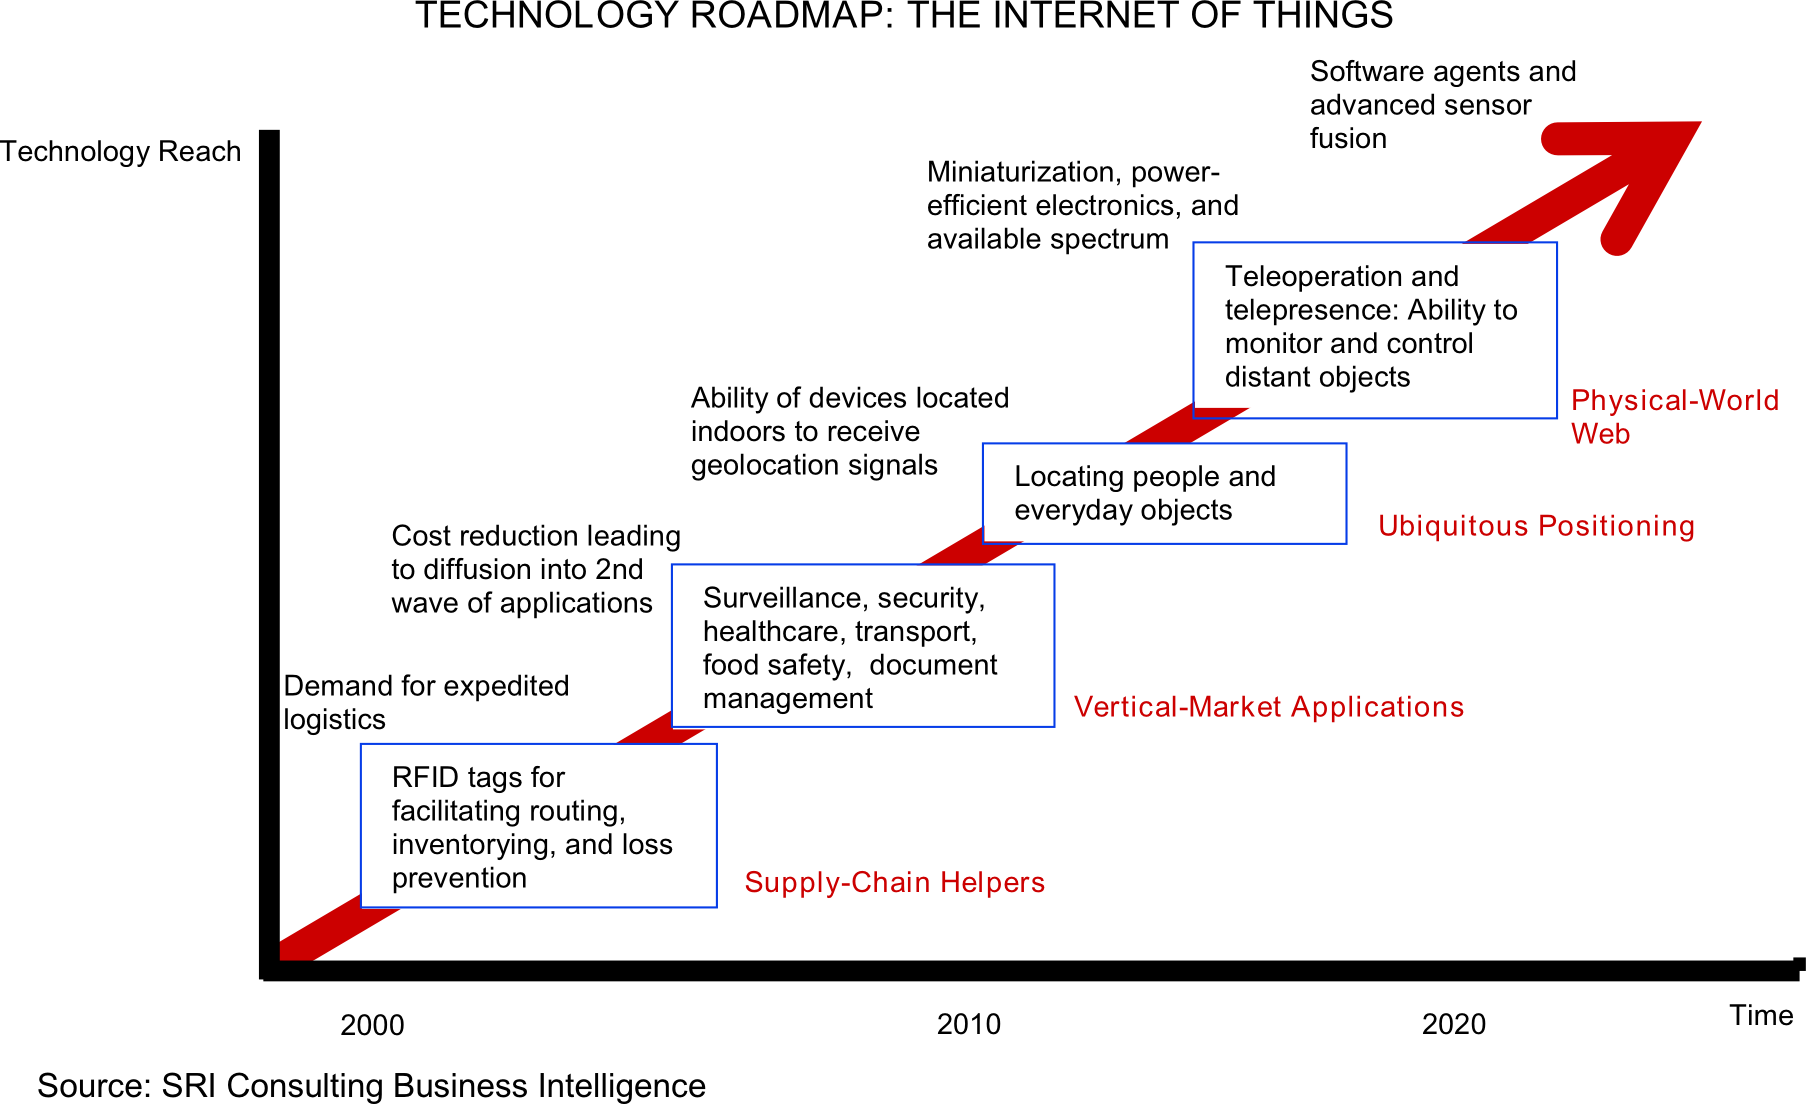
\includegraphics[width=\linewidth]{Internet_of_Things.png}
  \caption{Trend dell'internet of things}
  \centering
  \label{fig:trendIoT}
\end{figure}
Secondo le proiezioni di Gartner, Inc. una corporation per la ricerca e advisory tecnologica, entro il 2020 ci saranno oltre 20 miliardi di device connesse all'Internet of Things. Si sta parlando di una Industria 4.0 dove l'automazione industriale integra l'IoT per migliorare le condizioni di lavoro e la produttivit\`a. La chiave di volta dell'Industria 4.0 sono i sistemi ciberfisici (CPS), ovvero sistemi fisici che sono strettamente connessi con i sistemi informatici e possono interagire e collaborare con altri sistemi CPS i quali costituiscono lo step evolutivo successivo delle device IoT. 
Un altro settore nel quale si proiettano ulteriori sviluppi \`e la Big Data Analysis. L'ubiquit\`a dei dispositivi intelligenti connessi all'Internet delle Cose permette analisi di dati vastissimi ai quali precedentemente era impensabile avere accesso. Le informazioni che si possono ricavare da questi dati sono molteplici e di sicuro interesse per molti ambiti di applicazione.

%% Interruzione di pagina
\newpage

%% Classi di applicazioni IoT
\section{Classi di applicazioni IoT}
Passiamo ora ad analizzare i campi di applicazione pi\`u diffusi per l'Internet delle Cose.

%% Qui ho rubato da Wikipedia inglese il paragrafo sulle Applications nella pagina dedicata all'IoT
%% TODO: Cambiare un po' le parole in modo che non si capisca che ho copiato =D
\subsection{Environmental monitoring}
Le applicazioni di monitoraggio ambientale tipicamente utilizzano sensori collegati all'Internet delle Cose per fornire assistenza nella protezione dell'ambiente. Il monitoraggio pu\`o interessare la qualit\`a dell'aria o dell'acqua, condizioni atmosferiche o del suolo, e pu\`o includere aree come il monitoraggio degli spostamenti della fauna selvatica e del suo habitat. Ci\`o pu\`o avere applicazioni anche nell'ambito della rilevazione di disastri naturali: sistemi di allerta per terremoti e tsunami possono essere implementati nell'ambito IoT. Device IoT in questo campo di applicazione sono tipicamente dislocate su un'ampia area geografica possono anche essere mobili.

\subsection{Infrastructure management}
Il monitoraggio e il controllo di infrastrutture urbane come ponti, rotaie, wind-farms \`e un campo di applicazione chiave dell'IoT. L'infrastruttura IoT pu\`o essere usata per monitorare eventi o cambiamenti nelle condizioni strutturali che possono compromettere la sicurezza o aumentare i rischi. Pu\`o altres\`\i\ essere usato per la programmazione di interventi di manutenzione in maniera pi\`u efficiente coordinando le operazioni tra diversi fornitori di servizi. Le device IoT sono anche usate per controllare infrastrutture critiche come ponti per fornire accesso alle navi. Si pensa che l'utilizzo di device IoT possa migliorare la gestione degli incidenti e la coordinazione in caso emergenze, la qualit\`a del servizia e ridurre i costi in tutte le aree legate alla gestione delle infrastrutture.

\subsection{Manufacturing}
L'ambiente manifatturiero \`e sicuramente una delle applicazioni di punta dell'IoT fina dalla sua nascita. Gli inteventi dell'IoT spaziano dalla gestione degli equipaggiamenti al tracking degli asset nell'ambiente produttivo. Questa sinergia permette alle aziende di avere una maggior flessibilit\`a e di ottimizzare in tempo reale i sistemi di produzione nonch\`e la rete di approviggionamento grazie all'interconnesione tra macchinari, sensori e sistemi.
L'integrazione di sistemi IoT all'interno di catene di produzione permette la predictive maintenance, valutazione statistica della degradazione dello stato dei macchinari, e prevenzione di guasti.
Come visto in precedenza l'evoluzione dell'Industria 4.0 \`e interamente basata sull'integrazione tra sistemi di produzione e l'Internet of Things.

\subsection{Energy management}
L'intregrazione di reti di sensori e attutatori, connessi ad internet, si pensa possa ottimizzare il consumo energetico in ambito industriale e casalingo. L'integrazione di device IoT all'interno di contatori per l'energia, cos\`\i\ come dispositivi domestici e industriali, capaci di comunicare con le compagnie per la rete elettrica possono permettere una gestione migliore della generazione ed utilizzo dell'energia. Questo tipo di device inoltre permetterebbe agli utenti di controllare in remoto i loro dispositivi, o controllarli centralmente grazie a interfacce cloud, in modo tale da implementare funzioni avanzate come la programmazione delle accensioni o dell'utilizzo dei dispositivi. Questo tipo di applicazioni \`e molto diffuso nel campo della domotica, i termostati IoT sono un ottimo esempio di questa applicazione.

\subsection{Medical and Healthcare}
Device connesse all'Internet delle cose possono essere abilitare il monitoraggio remoto dello stato di salute e sistemi di notifica delle emergenze. Queste device per il rilevamento dello stato di salute possono variare dal rilevamento della pressione arteriosa fino al conteggio dei battiti del cuore. Alcuni ospedali hanno cominciato ad utilizzare "letti smart" in grado di rilevare quanto il letto \`e occupato e quando il paziente sta cercando di alzarsi. Ormai sono molto diffusi dispositivi per il tracciamento delle attivit\`a dell'utente che incoraggiano uno stile di vita salutare, in questo ambito rientrano le wearable device come i fitness trackers.

\subsection{Settore dei trasporti}
%% Qui mi ricollego al PCN che \`e la sezione seguente
L'IoT pu\`o dare assistenza nella integrazione delle comunicazioni, controlli e elaborazione delle informazioni attraverso vari sistemi di trasporto. Le applicazioni dell'IoT si estendono a tutti gli aspetti dei sistemi di trasporto: i veicoli, l'infrastruttura, il pilota e i passeggeri. L'interazione dinamica tra questi componenti permette una comunicazione inter e intra veicolare, controllo del traffico intelligente, smart parking, gestione della logistica e delle flotte, controllo dei veicoli e sicurezza stradale.
L'applicazione sviluppata nel corso della tesi \`e appunto legata a questo ambito di applicazione dell'IoT e nel prossimo paragrafo ne analizzeremo gli obiettivi e funzionalit\`a.

%% Interruzione di pagina
\newpage

%% Sezione PCN
\section{Passenger Counter}
Il Passenger Counter, o contatore di passeggeri, \`e un dispositivo IoT la cui funzione \`e quella di rilevare e conteggiare i passeggeri presenti all'interno di un sistema di trasporto pubblico. Esso deve altres\`\i\ fornire i dati in tempo reale al gestore del servizio, sfruttando l'Internet delle Cose, in modo tale che sia possibile:
\begin{itemize}
\item Rilevare frodi.
\item Aumentare l'efficienza della flotta di mezzi migliorando la gestione e la programmazione dei percorsi.
\item Restringere il numero di persone sul mezzo per ragioni di sicurezza.
\item Analizzare i flussi di traffico all'interno delle citt\`a.
\end{itemize}
Il dispositivo deve essere in grado di effettuare il conteggio in modo non invasivo e contact-less, tenendo conto delle restrizioni dovute all'ambiente nel quale deve essere applicato.

\begin{figure}[h!]
  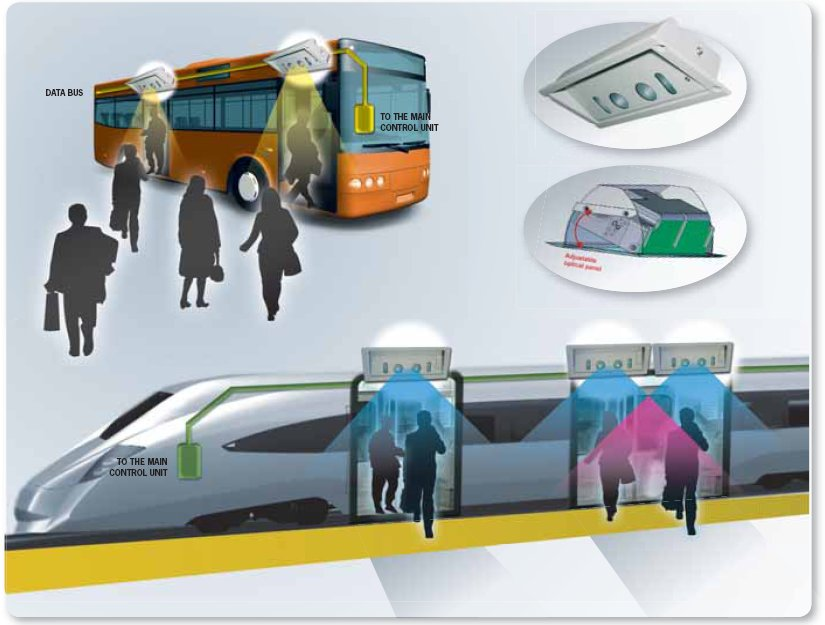
\includegraphics[width=9cm]{PassengerCountersz.jpg}
  \centering
  \caption{Schematizzazione del contatore di passeggeri}
  \label{fig:SchemPCN}
\end{figure}

Il lavoro presentato in questa tesi \`e stato commissionato da Eurotech: azienda dedicata alla ricerca, sviluppo e produzione di sistemi embedded e computer ad alte prestazioni e con sede ad Amaro. L'azienda inoltre ha una forte rilevanza in ambito IoT in quanto, oltre a fornire dispositivi IoT ready, ha realizzato una piattaforma Machine-to-Machine che consente ai dispositivi, ai sensori e a tutti i sistemi distribuiti sul campo di comunicare tra loro trasferendo le informazioni rilevanti alle business application ed alle infrastrutture IT. Il PCN o Passenger Counter \`e uno dei prodotti di punta dell'azienda ed \`e stato selezionato come progetto per questa tesi.

%% Interruzione di pagina
\newpage

\begin{figure}[h!]
  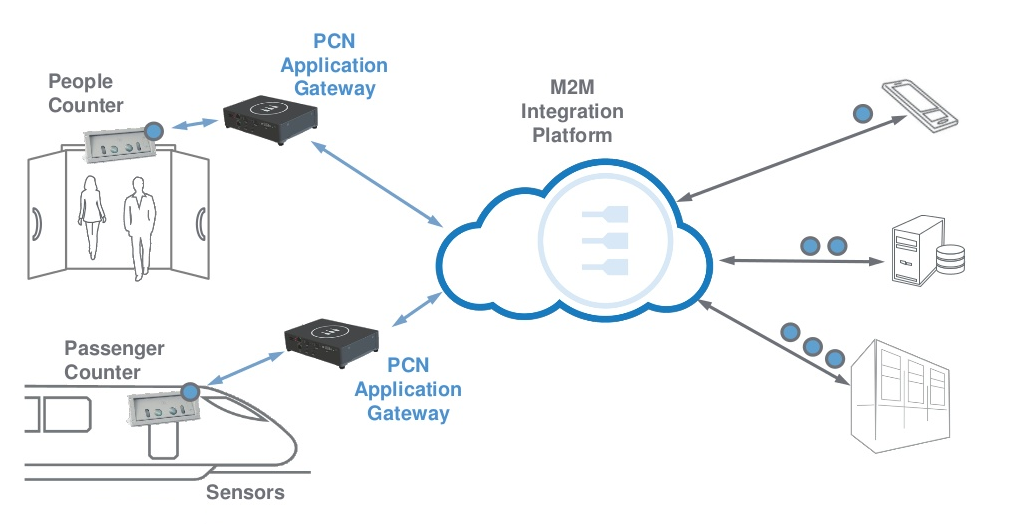
\includegraphics[width=\textwidth]{SchemaPCNIoT.png}
  \centering
  \caption{Schema Passenger Counter Eurotech}
  \label{fig:SchemPCNEurotech}
\end{figure}

Il sistema di conteggio di passeggeri consta di tre parti fondamentali come schematizzato in figura \ref{fig:SchemPCNEurotech}:
\begin{enumerate}
\item Dispositivo di acquisizione video.
\item Dispositivo di elaborazione e trasmissione dei dati in real-time.
\item Infrastruttura di rete cloud per il raccoglimento dei dati.
\end{enumerate}
\`E quindi possibile accedere ai dati raccolti da pi\`u dispositivi per mezzo della piattaforma M2M proprietaria di Eurotech.

%% Interruzione di pagina
\newpage

\section{Obiettivi della tesi}
L'obiettivo della tesi \`e stato quello di realizzare una nuova versione del Passenger Counter di Eurotech basandosi sulla infrastruttura software/hardware fornita dall'azienda, cercando di migliorare quanto gi\`a fatto da Eurotech, esplorando soluzioni tecnologiche alternative. Questo obiettivo \`e stato quindi suddiviso in tre parti:
\begin{enumerate}
\item Identificare gli ambienti di sviluppo pi\`u idonei alla realizzazione del progetto.
\item Realizzare una nuova versione del Passenger Counter puntando a migliorare le prestazione ed abbattere i costi, adattandolo alle tecnologie usate dall'azienda per i suoi prodotti. 
\item Realizzare una infrastruttura software che fornisse tutti gli strumenti e le librerie necessarie all'implementazione del Passenger Counter realizzato e che potesse essere installato sulla piattaforma hardware fornita da Eurotech.
\end{enumerate}

% TODO: Attenzione! Aggiornare questa sezione ad ogni cambiamento della struttura del testo. (Se ce ne sono).
\section{Struttura della tesi}
Qui di seguito \`e riportata l'organizzazione del testo:
\begin{itemize}
\item Capitolo 1: Introduzione al contesto dell'Internet of Things e all'applicazione di conteggio dei passeggeri.
\item Capitolo 2: Analisi della versione corrente del Passenger Counter realizzato da Eurotech. Segue una trattazione dettagliata delle tecnologie e software utilizzati nella realizzazione del progetto.
\item Capitolo 3: Descrizione degli step intrapresi per lo sviluppo. Si suddivide in tre sezioni principali:
    \begin{itemize}
    \item Analisi degli ambienti disponibili per l'image processing embedded e motiviazioni per le quali si \`e deciso quello che \`e stato utilizzato.
    \item Implementazioni e confronti delle versioni realizzate per il contatore dei passeggeri.
    \item Realizzazione e features della distribuzione Linux realizzata a supporto del progetto
    \end{itemize}
\item Capitolo 4: Conclusioni
\end{itemize}

%% Capitolo 2: Contesto tecnologico di dettaglio
\chapter{Contesto tecnologico di dettaglio}
Passiamo ora a descrivere pi\`u tecnicamente e nel dettaglio le tecnologie utilizzare nello svolgimento della tesi.

\section{Tecnologie PCN Eurotech}

\begin{figure}[h!]
  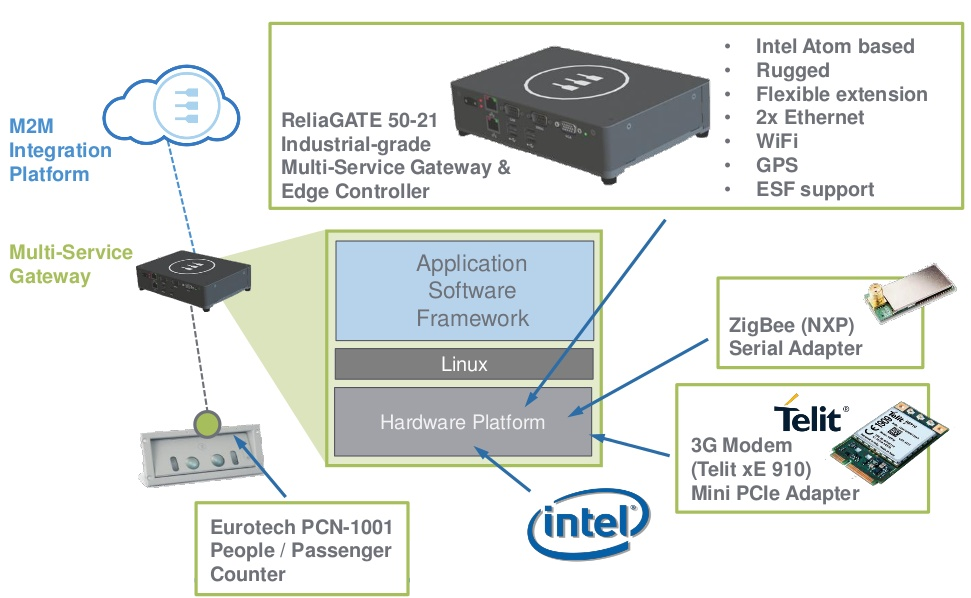
\includegraphics[width=\textwidth]{StrutturaPCN.png}
  \centering
  \caption{Struttura del Passenger Counter di Eurotech}
  \label{fig:PCNEurotechHardware}
\end{figure}

%% Interruzione di pagina
\newpage

\subsection{Hardware}
Il sistema di conteggio dei passeggeri consta di due componenti hardware fondamentali: il gateway e il dispositivo di acquisizione delle immagini.

Il gateway \`e un'altro prodotto della Eurotech noto come ReliaGATE 50-21. Utilizza un processore x86 Intel Atom Z510P al quale sono state aggiunte opportune interfacce di rete per il deployment mobile. Esso ha infatti interfacce 2G/3G, WiFi, 802.15.4/Zigbee e GPS. Questo componente rappresenta l'unit\`a di elaborazione centrale del sistema nonch\`e il mezzo attraverso il quale i dati di conteggio vengono raccolti e trasmessi alla piattaforma cloud della Eurotech.

\begin{figure}[h!]
  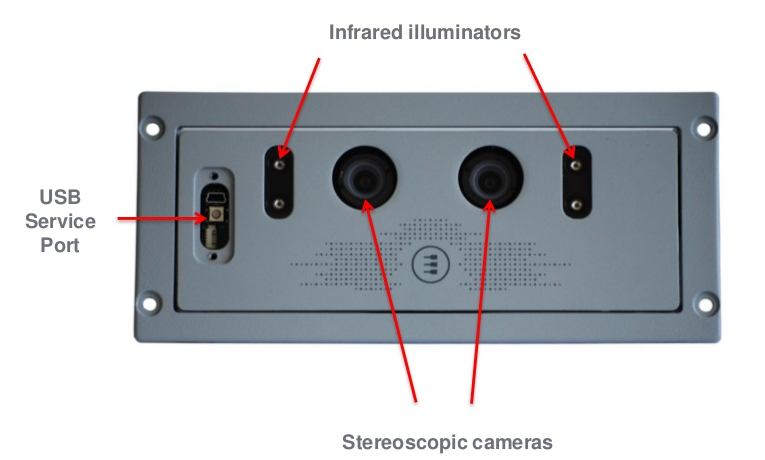
\includegraphics[width=\textwidth]{DispositivoAcquisizioneImmagini.png}
  \centering
  \caption{Dispositivo di acquisizione delle immagini 3D}
  \label{fig:DispAcqImm3D}
\end{figure}

Il dispositivo di acquisizione video visibile in figura \ref{fig:DispAcqImm3D}. Esso nasconde al suo interno una FPGA programmata con una IP proprietaria Eurotech che permette la ricostruzione in 3D delle immagini acquisite dalle telecamere stereoscopiche di cui \`e dotato il dispositivo.
Il funzionamento \`e il seguente: i proiettori di luce infrarosse illuminano la scena, le telecamere a infrarossi stereoscopiche acquisiscono le immagini nello spettro della luce infrarossa. Le due immagini vengono passate alla FPGA che per mezzo di tecniche di ricostruzione stereoscopica accelerate in hardware permette di generare delle immagini in scala di grigi dove l'informazione di profondit\`a \`e data dal colore del pixel. Queste immagini vengono quindi passate all'unit\`a di elaborazione centrale che vi applica un semplice algoritmo per il tracciamento dei passeggeri di cui discuteremo il funzionamento nel dettaglio nel prossimo paragrafo.

%% Interruzione di pagina
\newpage

\subsection{Algoritmo per il tracciamento dei passeggeri}

\begin{figure}[h!]
  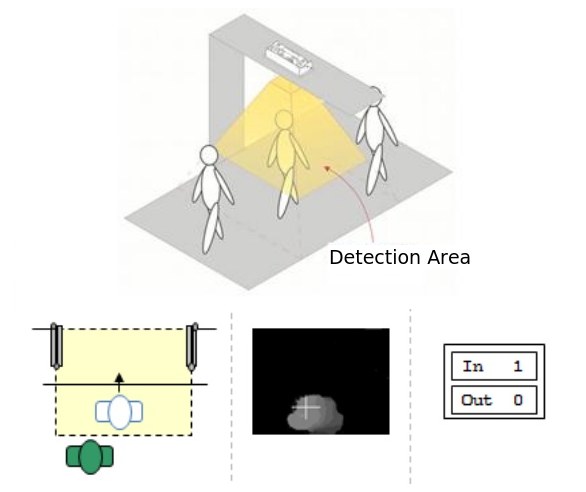
\includegraphics[scale=0.75]{Algoritmov2.png}
  \centering
  \caption{Schematizzazione funzionamento algoritmo tracciamento passeggeri}
  \label{fig:SchemAlgrTrackPCNEurotech}
\end{figure}

%% TODO: Chiedere al prof se il conteggio viene effettuato sul ReliaGate o sul DynaPCN
L'unit\`a di elaborazione centrale si vede arrivare in ingresso una immagine in scala di grigi in cui \`e codificata l'informazione di profondit\`a tramite il colore dei pixel. I punti pi\`u vicini al rilevatore tendono al bianco, i punti pi\`u lontani tendono al nero.
Il cuore dell'algoritmo opera come segue:
\begin{enumerate}
\item Vengono rilevati i massimi locali all'interno dell'imagine in scala di grigi, i quali rappresentano le teste delle persone.
\item Traccia la posizione nel tempo di questi massimi locali all'interno del flusso di immagini.
\item Rileva quando questi massimi locali attraversano una linea di demarcazione virtuale, la quale indica l'ingresso o uscita dalla soglia e aggiorna i contatori.
\end{enumerate}
In figura \ref{fig:SchemAlgrTrackPCNEurotech} \`e riportata una schematizzazione di quanto accade durante il conteggio.

%% Interruzione di pagina
\newpage

\subsection{Infrastruttura software}

\begin{figure}[h!]
  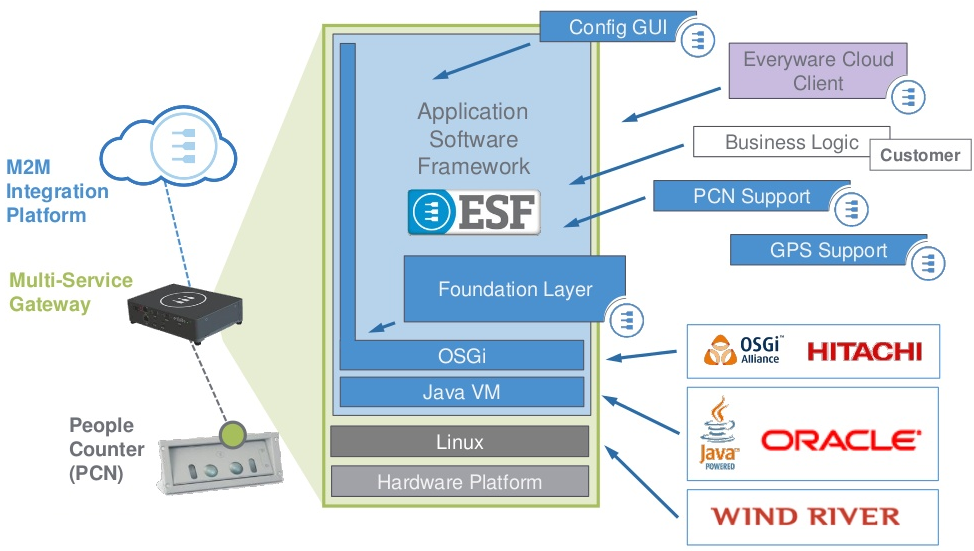
\includegraphics[width=\textwidth]{SoftwareStack.png}
  \centering
  \caption{Schematizzazione stack software del sistema di Passenger Counting}
  \label{fig:StackSoftwarePCNEurotech}
\end{figure}

La piattaforma sulla quale si basa il Passenger Counter Eurotech \`e basata su una distribuzione custom di Linux realizzata per mezzo del progetto Yocto (Per affrondimenti circa questo strumento si veda il paragrafo \ref{Yocto}). Ad essa sono stati aggiunti i driver proprietari per le tecnologie Eurotech. Sopra di essa \`e presente la Java Virtual Machine la quale permette l'esecuzione del framework OSGi (Per affrondire questo framework si veda il paragrafo \ref{OSGi}). Su OSGi \`e basato il framework proprietario di Eurotech: Everyware Software Framework (ESF). Esso permette il deployment di applicazioni del cliente in modo flessibile tramite interfaccia grafica da web, la quale \`e resa disponibile dall'infrastruttura M2M di Eurotech.
Nei prossimi capitoli vedremo come sia stato necessario adattare l'applicazione realizzata nel corso di questa tesi alla infrastruttura qui descritta, nonch\`e modificare parte dell'infrastruttura per aggiungere funzionalit\`a mancanti e necessari alla nuova versione del Passenger Counter.

%% Interruzione di pagina
\newpage

\subsection{Problematiche di questa soluzione}
Questo sistema di conteggio dei passeggeri non \`e per\`o esente da problematiche, le quali sono state il punto di partenza per il mio lavoro. Le principali sono le seguenti:

\begin{enumerate}
\item Le ottiche del dispositivo di acquisizione delle immagini sono costose e difficili da reperire.
\item L'utilizzo di una FPGA per la ricostruzione delle informazioni di profondit\`a fa aumentare i costi di produzione.
\item Per come \`e stata implementata la soluzione \`e necessario installare una unit\`a computazionale per dispositivo di acquisizione delle immagini. Anche questo contribuisce ad aumentare i costi di produzione di un sistema PCN.
\end{enumerate}

Vedremo che nella versione del Passenger Counter realizzata nel corso di questa tesi sono stati risolti in buona parte tutte queste problematiche, con vari gradi di successo.

%% Interruzione di pagina
\newpage

\section{Tecnologie utilizzate durante lo sviluppo della tesi}
In questa sezione andremo ad esaminare le tecnologie che sono state utilizzate per realizzare la nuova versione del Passenger Counter.

%%TODO: Aggiungere nella bibliografia i riferimenti ai Datasheet delle telecamere
\subsection{Telecamere Intel RealSense}
Come dispositvi di acquisizione delle immagini sono state utilizzate le telecamere Intel RealSense. Esse sono telecamere ad infrarossi di nuova generazione che permettono la ricostruzione delle informazioni di profondit\`a della scena filmata sfruttando diverse tecniche di elaborazione delle immagini.

\subsubsection{Intel RealSense R200}

\begin{figure}[h!]
  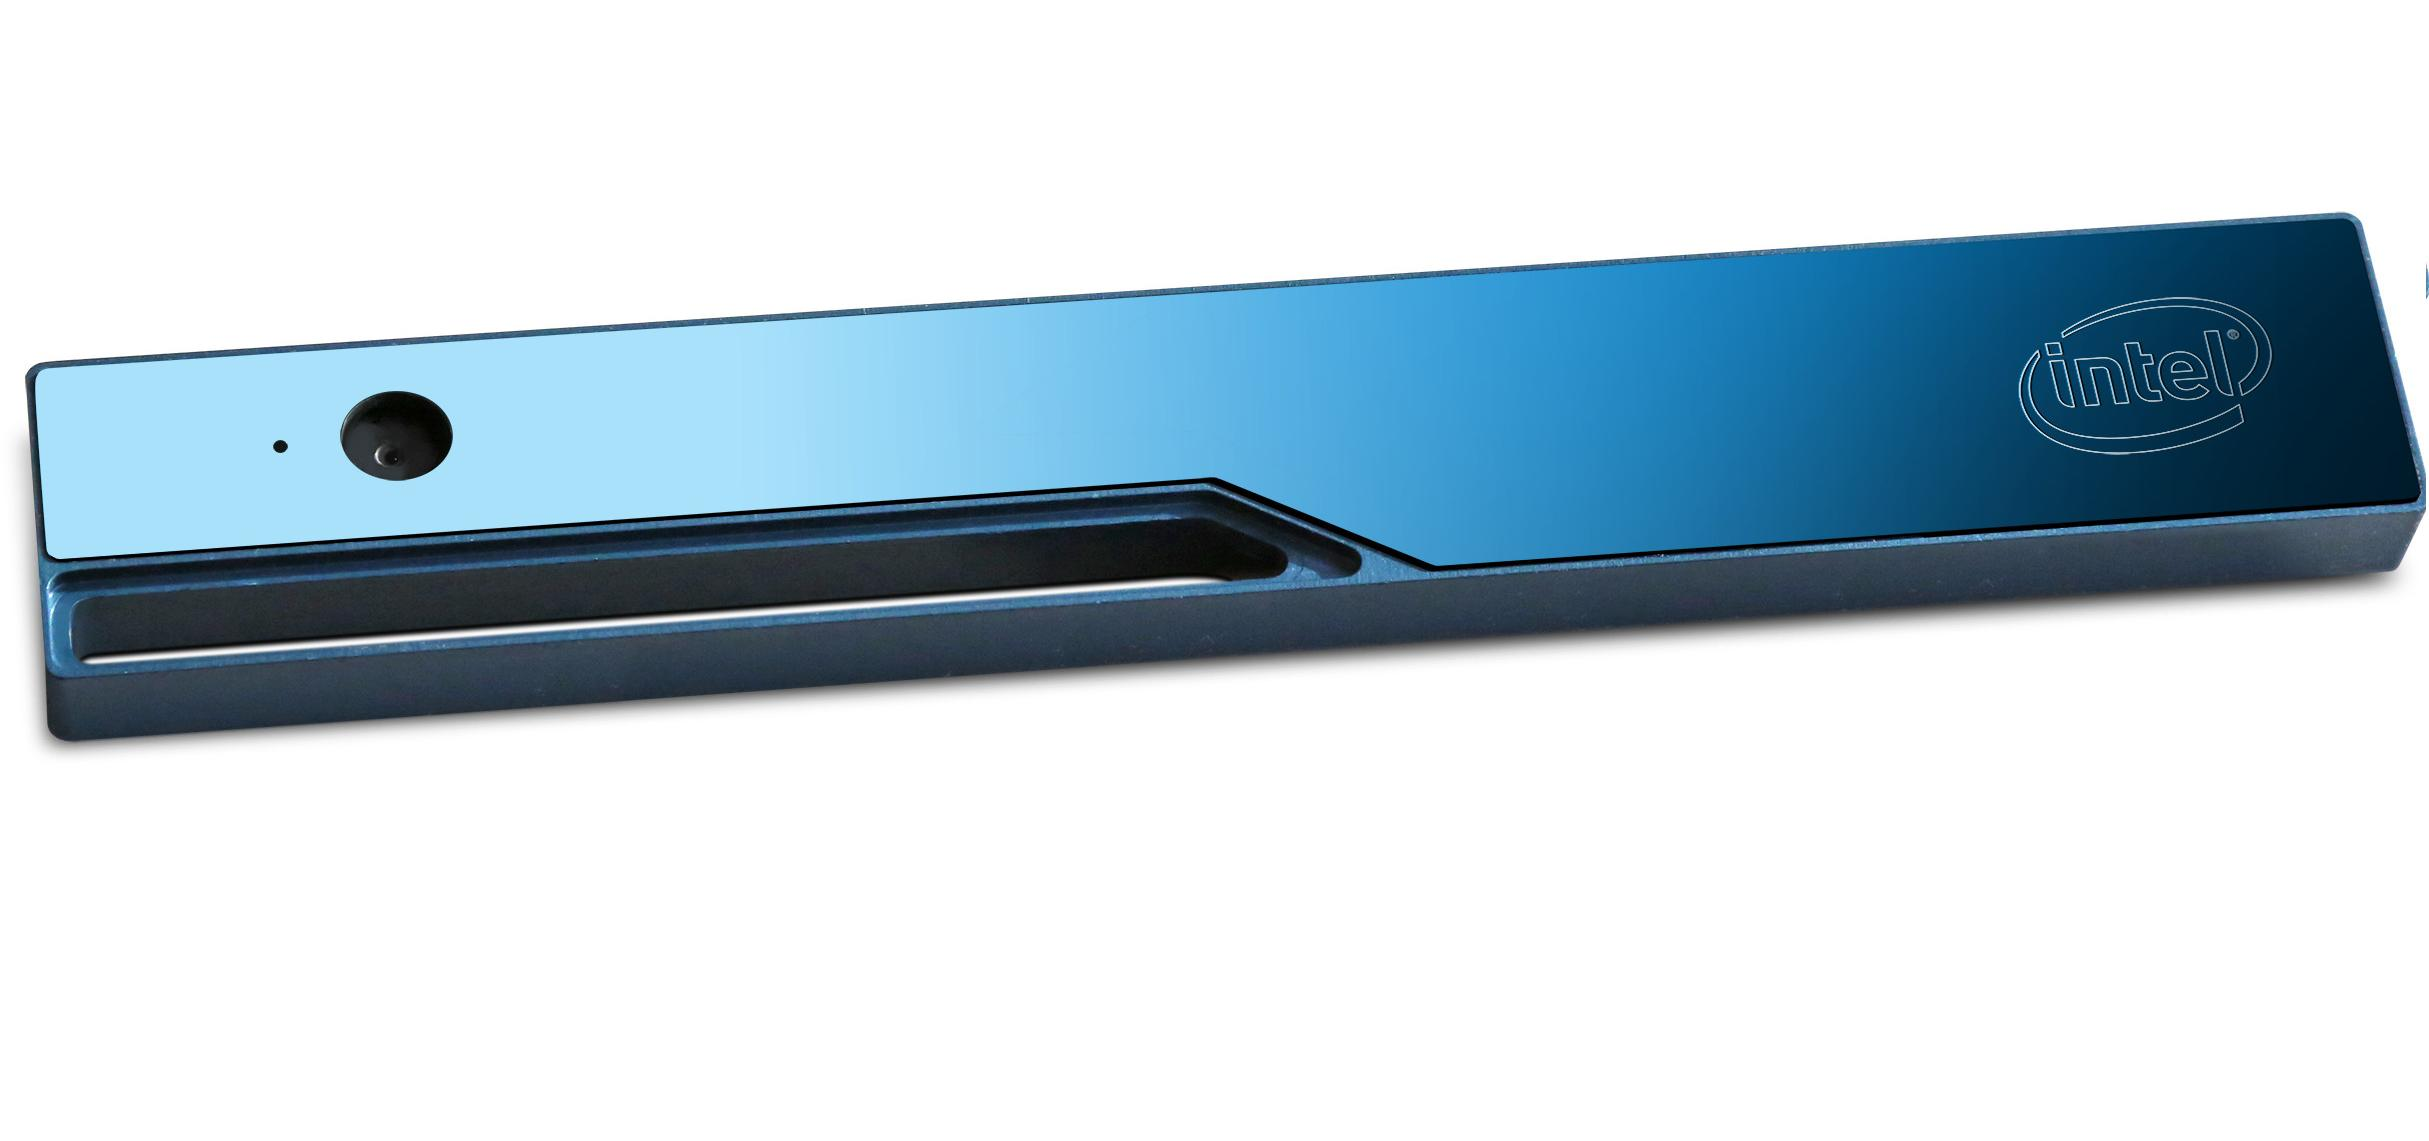
\includegraphics[width=.49\textwidth]{R200.jpg}
  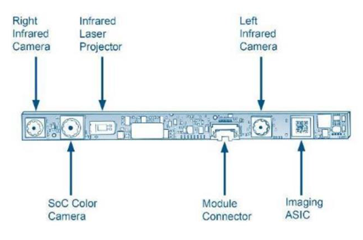
\includegraphics[width=.49\textwidth]{r200_module.png}
  \centering
  \caption{Telecamera R200}
  \label{fig:R200}
\end{figure}

Il funzionamento di queste telecamere \`e lo stesso del Passenger Counter Eurotech. Sul modulo sono presenti due illuminatori ad infrarossi che illuminano la scena. Due telecamere stereoscopiche acquisiscono due immagini leggermente diverse dovute al diverso posizionamento delle telecamere. Analizzando le differenze tra le due immagini per mezzo di algoritmi di image processing ricostruiscono l'informazione di profondit\`a. Per ottenere una ricostruzione delle informazioni in real-time \`e stato usato un circuito ASIC che garantisse le prestazioni desiderate. Il funzionamento \`e riassunto in figura \ref{fig:SchemaFunzR200}.

\begin{figure}[h!]
  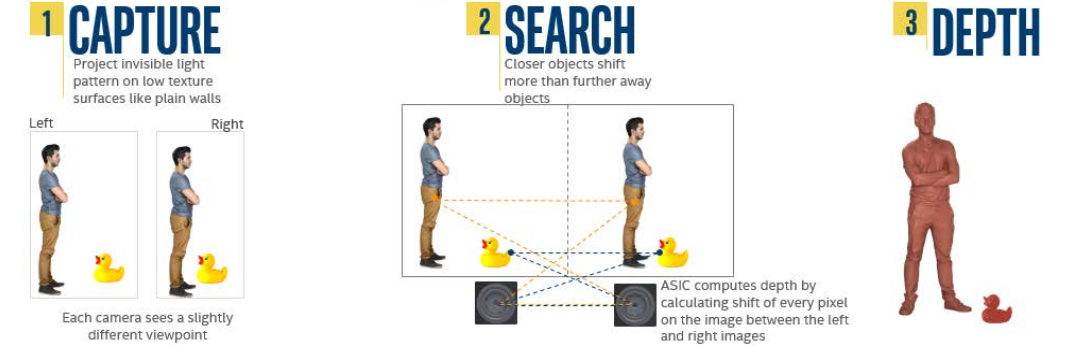
\includegraphics[width=\textwidth]{DepthDataFlowR200.png}
  \centering
  \caption{Schema funzionamento Intel RealSense R200}
  \label{fig:SchemaFunzR200}
\end{figure}

Specifiche tecniche:

\begin{table}[h!]
    \centering
	\begin{tabular}{|c|c|c|}
	\hline
	& Depth Stream & Color Stream \\ \hline
	Risoluzione massima & 640 x 480 & 1920 x 1080 \\ \hline
    Frame rate massimo & 90fps & 60fps \\ \hline
    FOV (WxH) & 56 x 43 & 70 x 43 \\ \hline
    Indoor Range & 0.7 - 3.5m & - \\ \hline
    OutdoorRange & 10m & - \\
    \hline
	\end{tabular}
    \caption{Specifiche tecniche Intel RealSense R200}
\end{table}

%% Interruzione di pagina
\newpage

\subsubsection{Intel RealSense SR300}

\begin{figure}[h!]
  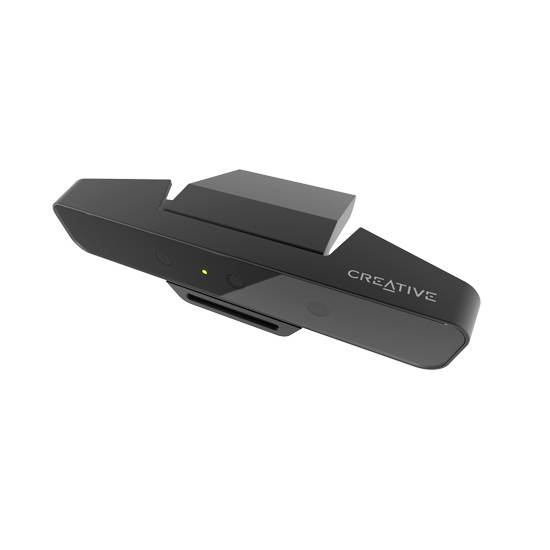
\includegraphics[width=.49\textwidth]{SR300.jpg}
  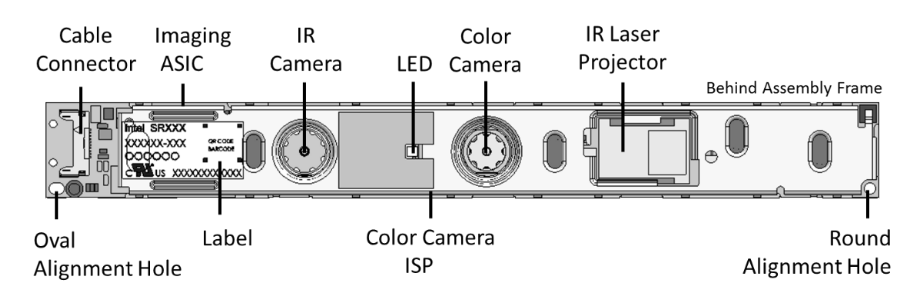
\includegraphics[width=.49\textwidth]{SR300_module.png}
  \centering
  \caption{Telecamera SR300}
  \label{fig:SR300}
\end{figure}

La telecamera S300 utilizza una tecnica di rilevamento tridimensionale nota come luce strutturata. Il proiettore presente sul modulo proietta un pattern noto sulla scena. La deformazione dell'immagine proiettata permette ai sistemi di visione di calcolare la profondit\`a degli oggetti colpiti ed ottenere altre informazioni sulla superficio. L'acquisizione delle immagini a infrarossi in questo caso viene effettuata da un singolo scanner 3D a luce strutturata. In figura \ref{fig:SchemaFunzSR300} \`e schematizzato il funzionamento della telecamera.
Anche i questo caso l'informazione di profondit\`a viene ricostruita utilizzando un circuito ASIC.

\begin{figure}[h!]
  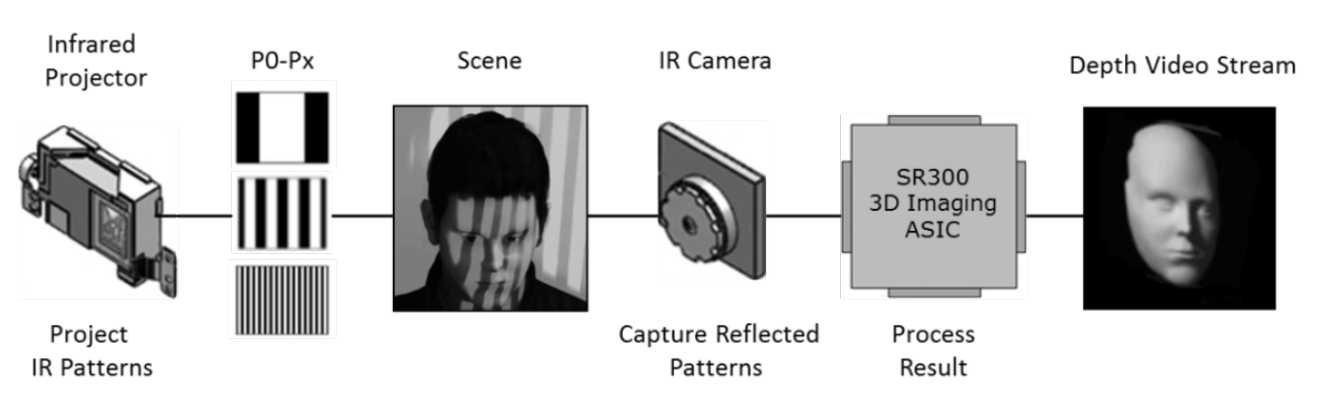
\includegraphics[width=\textwidth]{DepthDataFlowSR300.png}
  \centering
  \caption{Schema funzionamento Intel RealSense SR300}
  \label{fig:SchemaFunzSR300}
\end{figure}

%% Interruzione di pagina
\newpage

Specifiche tecniche:

\begin{table}[h!]
    \centering
	\begin{tabular}{|c|c|c|}
	\hline
	& Depth Stream & Color Stream \\ \hline
	Risoluzione massima & 640 x 480 & 1920 x 1080 \\ \hline
    Frame rate massimo & 60fps & 60fps \\ \hline
    FOV (WxH) & 71 x 55  & 68 x 41 \\ \hline
    Indoor Range & 0.2 - 1.5m & - \\ \hline
    OutdoorRange & - & - \\
    \hline
	\end{tabular}
    \caption{Specifiche tecniche Intel RealSense SR300}
\end{table}

\subsubsection{Libreria librealsense e formato immagine}
Per l'interfacciamento software la Intel fornisce una libreria in C++ tramite la quale \`e possibile recuperare i frame dalle telecamere: la libreria \textbf{librealsense}\footnote{Repository libreria all'indirizzo: https://github.com/IntelRealSense/librealsense}. Essa provvede all'inizializzazione delle telecamere, apertura dei vari stream disponibili, impostazione di risoluzione e framerate. Gli stream disponibili sono: le immagini a colori, le immagini della telecamera a infrarossi e le immagini in cui \`e codificata l'informazione di profondit\`a. Nonostante usino tencologie diverse entrambe le telecamere forniscono lo stesso formato in uscita.

Lo stream di profondit\`a \`e uno stream di immagini a 16 bit privi di segno in cui il valore di ogni pixel rappresenta la distanza dalla telecamera. La distanza \`e fornita a meno di un fattore di scala reperibile per mezzo di una semplice chiamata di funzione. \`E possibile quindi risalire alla distanza in metri di un pixel dalla telecamera semplicemente moltiplicando il valore del pixel per il fattore di scala.
Vi \`e una eccezione a questa codifica in quanto, il valore del pixel 0, \`e attribuito ai pixel per i quali non \`e stato possibile ricavare informazione sulla distanza, ci\`o pu\`o essere dovuto a problemi di range o esposizione dell'immagine.

Vi sono per\`o delle minime differenze tra le due telecamere per quanto riguarda la risoluzione della distanza calcolata:
\begin{itemize}
\item Per la Intel RealSense SR300: il formato dello stream di profondit\`a \`e di 16 bit privi di segno interpolati su un range di 8m nonostante il range della telecamere arrivi ad un massimo di 1,5m. Ci\`o implica che la risoluzione della profondit\`a sia 0,125mm. 
\item Per la Intel RealSense R200: il formato \`e di 16 bit privi di segno interpolati su un range di circa 65m. Ci\`o implica una risoluzione di profondit\`a di 1mm.
\end{itemize}
Questo fatto non ha per\`o comportato problemi dal punto di vista della funzionalit\`a dell'applicazione in quanto la risoluzione e precisione delle telecamere non \`e critica per il corretto funzionamento del contatore.

%% Interruzione di pagina
\newpage

%% Copiato spudoratamente dalla mia presentazione su OpenCV.
\subsection{Libreria per l'image processing: OpenCV}\label{OpenCV}
Siccome una parte centrale della tesi verteva sull'elaborazione delle immagini \`e stato necessario integrare nel progetto l'uso della libreria OpenCV, ormai standard de facto nell'ambito dell'elaborazione delle immagini.

OpenCV, acronimo di Open Source Computer Vision, \`e una libreria software multipiattaforma finalizzata all'image processing real-time e alla computer vision. La libreria \`e rilasciata tramite licenza Berkeley Software Distribution (BSD) quindi \`e ad uso gratuito sia per fini accademici che commerciali. Contiene pi\`u di 2500 algoritmi pre-ottimizzati per le operazioni di image processing, comupter visione e machine learning pi\`u comuni. Sviluppata in C/C++, \`e dotata di interfacce verso C, Python, Java e MATLAB. Poich\`e finalizzata all'utilizzo real-time, la libreria sfrutta molteplici interfacce per l'accelerazione hardware (CUDA, OpenCL, Intel Integrated Perfomance Primitives). OpenCV ha una struttura modulare, il che significa che il pacchetto include diverse librerie statiche o condivise.

\subsubsection{Moduli principali e finalit\`a}
\begin{itemize}
\item \textbf{Modulo core}: funzionalit\`a di base. Lo scopo del modulo \`e  definire interfacce e funzionalit� che permettano di semplificare la manipolazione di immagini e flussi video. Il modulo contiene le funzionalit� di  base delle libreria e ne definisce le strutture fondamentali nonch\'e gestisce la memoria. 
\item \textbf{Modulo highui}: High-level GUI e Media I/O. l modulo HighGUI \`e stato progettato per fornire funzioni che permettano di provare le funzionalit\`a della libreria ed osservare i risultati velocemente. Fornisce semplici interfacce per creare e manipolare finestre che possano visualizzare immagini e aggiungere slider alle finestre, gestire semplici eventi come click del mouse e comandi da tastiera.
\item \textbf{Modulo imgproc}: image processing. Il modulo di Image Processing contiene funzioni e classi per la manipolazione di immagini. Ci\`o comprende:
    \begin{itemize}
    \item Image Filtering: funzioni per la convoluzione di immagini con un kernel, dilatazione di immagini, filtro Sobel, GaussianBlur ecc...
    \item Trasformazioni geometriche: ridimensionamenti, warping ecc...
    \item Funzioni per il disegno: permettono di disegnare semplici forme sulle immagini che vengono manipolate
    \item Funzioni per l'analisi delle immagini: istogrammi, analisi strutturale e descrittori di forme, motion analysis e tracking di oggetti.
    \end{itemize}
\item \textbf{Modulo videoio}: lettura e scrittura di file, nonch\`e analisi di video. Le funzioni principali implementate sono: analisi del movimento, sottrazione del background, rilevamento e tracciamento di oggetti.
\item \textbf{Modulo objdetect}: rilevazione di oggetti. Implementa funzioni e classi per il rilevamento e tracciamento di oggetti all'interno di immagini e flussi video. OpenCV ottiene tutto ci\`o facendo leva sui Haar Feature-based Cascade Classifier e Histogram of Oriented Gradients object detector.
\item \textbf{Modulo ml}: machine learning. La Machine Learning Library (MLL) \`e un insieme di classi e funzioni per la classificazione statistica, regressione e clustering dei dati. La maggior parte degli algoritmi di classificazione e regressione sono implementati come classi C++. Algoritmi implementati dal modulo:
    \begin{itemize}
    \item Artificial Neural Networks / Multi-Layer Perceptrons.
    \item Tree Classifier.
    \item Expectation Maximization algorithm.
    \item K-nearest Neighbors model.
    \item Logistic Regression.
    \item Normal Bayes Classifier.
    \item Support Vector Machines (SVM).
    \item Random forest predictor.
    \item Sochastic Gradient Descent SVM classifier.
    \end{itemize}
\end{itemize}

La struttura fondamentale della libreria \`e l'oggetto Mat, il quale \`e usato come contenitore delle immagini. Esso \`e una classe C++ formata da due componenti principali
\begin{itemize}
\item L'header: contenente informazioni come la dimensione della matrice, il metodo usato per salvarla, l'indirizzo dove \`e salvata ed un puntatore alla matrice.
\item La matrice: contenente i valori dei pixel dell'immagine la cui dimensionalit\`a dipende dal metodo utilizzato per salvare l'immagine (B/N, RGB ecc...)
\end{itemize}
Questa struttura \`e la stessa per tutti i tipi di immagine, indipendentemente dal formato nella quale \`e salvata. Questa astrazione facilita notevolmente la manipolazione delle immagini in quanto ci si riconduce velocemente ad una matrice di pixel manipolabile questa conversione \`e garantita dal modulo imgcodecs, la quale funzione non \`e altro che recuperare i dati sui pixel dell'immagine sulla quale si sta lavorando e generare i metadati per il tipo Mat.

\subsubsection{Storia}
Lanciato ufficialmente nel 1999, il progetto OpenCV era parte di una iniziativa Intel finalizzata all'avanzamento delle applicazioni CPU-intensive che includeva ray tracing real-time e display 3D. Inizialmente le finalit\`a del progetto erano descritte come:
\begin{itemize}
\item Permettere l'avanzamento della computer vision fornendo non solo una libreria di codice open-source ma anche pre ottimizzato per costruire l'infrastruttura base di applicazioni di computer visione.
\item Condividere conoscenza sulla computer vision fornendo una infrastruttura comune sulla quale tutti gli sviluppatori potessero costruire.
\item Far avanzare le applicazioni commerciali basate sulla computer vision rendendo il codice portabile, ottimizzato per le performance.
\end{itemize}
Ad oggi il supporto al progetto \`e dato dall'organizzazione no-profit OpenCV.org, la quale mantiene uno sviluppatore e un sito per la documentazione. La libreria \`e ormai lo standard de facto per le applicazioni di computer vision e image processing, vista la sua diffusione e la community molto attiva.

Per lo sviluppo dell'applicazione di Passenger Counter la scelta di utilizzare questa libreria \`e stata quasi obbligata visto l'ottimo supporto e diffusione della libreria. Inoltre la vasta portabilit\`a e l'attenzione alle performance la rendono particolarmente adatto al caso embedded real-time.

%% Interruzione di pagina
\newpage

%% TODO: Rivedi cosa hai scritto e amplia ancora se riesci
\subsection{Ambiente di sviluppo per l'OS: Yocto Project}\label{Yocto}
Per integrare nella piattaforma target gli strumenti necessari al funzionamento dell'applicativo \`e stato necessario realizzare una distribuzione Linux customizzata adatta alle nostre esigenze. Per farlo \`e stato utilizzato il progetto Yocto, standard industriale de facto per realizzare distribuzioni Linux embedded.

Yocto Project \`e un insieme di strumenti open source finalizzati alla creazione di distribuzioni Linux per sistemi embedded, corredate da toolchain di cross-compilazione ed emulatori, che siano indipendenti dall'architettura hardware. Yocto Project \`e quindi un ombrello sotto il quale si raccolgono vari sotto-progetti volti allo sviluppo di sistemi Linux embedded.

Le architettura supportate dal progetto sono le pi\`u diffuse nell'ambito embedded: ARM, MIPS, PowerPC e x86/x86-64. Una parte fondamentale di questo progetto \`e il build system open source basato sull'architettura OpenEmbedded. Questa implementazione di OpenEmbedded \`e chiamata Poky.

OpenEmbedded \`e framework software usato per creare distribuzioni Linux embedded. Il build system \`e basato sulle ricette BitBake le quali sono degli script bash specializzati che automatizzano la compilazione e la installazione di pacchetti software. Le ricette BitBake consistono di un URL che punta alla sorgente del pacchetto software, dipendenze e opzioni di compilazione ed installazione. Durante il processo di build sono usate per tenere traccia delle dipendenze ed effettuare cross-compilazione dei pacchetti affinch\`e sia possibile installarli sulla target distribution. BitBake stesso \`e uno dei componenti fondamentali di Yocto Project: \`e un build automation software, ovvero un tool che legge dei metadati sottoforma di "ricette" ed esegue task in base a dette ricette.

\subsubsection{Componenti del progetto Yocto}
\begin{itemize}
\item OpenEmbedded: \`e un build framework per embedded Linux. Permette la creazione di distribuzioni Linux complete per sistemi immersi e offre un ambiente di cross-compilazione completo. Il build system \`e basato su ricette BitBake.
\item BitBake: \`e un build automation software, ovvero un tool che legge dei metadati sottoforma di "ricette" ed esegue task in base a dette ricette. \`e uno dei componenti fondamentali di Yocto Project.
\item Poky: \`e una reference distribution di Yocto Project. Contiene l'OpenEmbedded Build System(BitBake e OpenEmbedded) assieme a un insieme di metadati che permettono di cominciare a costruire la propria distribuzione Linux embedded customizzata.
\item Layers: il build system del progetto Yocto \`e composto da layer. I layer sono una collezione logica di ricette che rappresentano stack di applicazioni o Board Support Packaged (BSP). I BSP contengono i pacchetti e i driver fondamentali necessari per costruire una distribuzione Linux per una specifica board o architettura. Solitamente questi BSP sono mantenuti dai produttori dell'hardware e sono l'interfaccia tra l'OS e l'hardware che lo esegue.
\end{itemize}

%% Interruzione di pagina
\newpage

\begin{figure}[h!]
  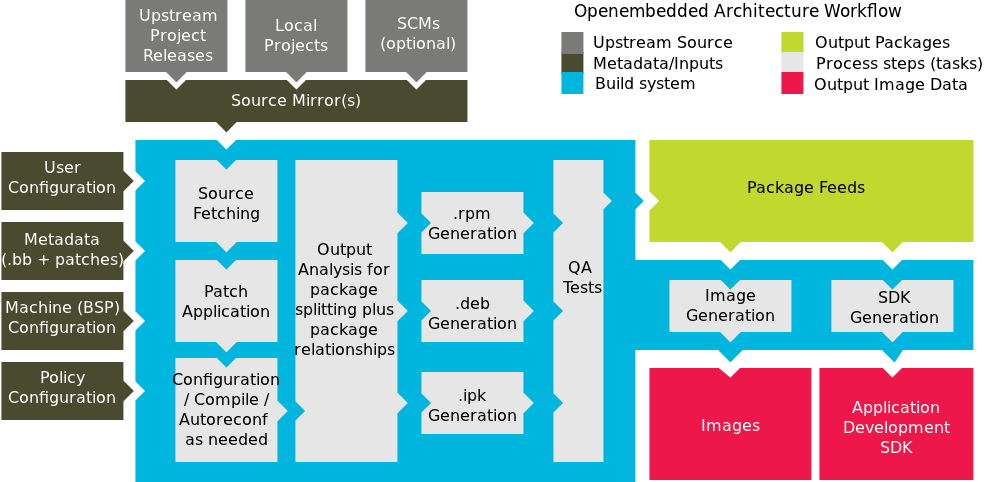
\includegraphics[width=\textwidth]{yocto-environment.png}
  \centering
  \caption{Workflow progetto Yocto}
  \label{fig:WorkflowYocto}
\end{figure}

\subsubsection{Processo di build di una distribuzione}
Dopo aver configurato e lanciato il processo di build il build system provvede ad eseguire le seguenti operazioni per ogni pacchetto e applicazione che si desidera installare:
\begin{enumerate}
\item Recupera autonomamente i sorgenti remoti e locali.
\item Procede alla cross-compilazione dei sorgenti.
\item Genera i file .deb/.rpm/.ipk dipendentemente dalla configurazione.
\end{enumerate}
Una volta che sono stati generati tutti i pacchetti richiesti procede alla generazione dell'immagine della distribuzione, genera quindi il filesystem, installa i pacchetti e genera l'immagine che pu\`o essere eseguita sulla macchina target. In seguito \`e possibile generare la toolchain per la cross-compilazione di sorgenti per l'immagine della macchina target, questo processo generer\`a un piccolo installer il quale installer\`a la toolchain nella macchina dedicata allo sviluppo delle applicazioni per la piattaforma target.

%% Interruzione di pagina
\newpage

Per lo sviluppo dell'applicazione del Passenger Counter \`e stato necessario realizzare l'immagine della distribuzione Linux opportunamente modificata e la toolchain di cross-sviluppo prima di cominciare lo sviluppo dell'applicazione. Una volta completati questi passaggi si \`e potuti passare allo sviluppo dell'applicazione sulla SDKMachine. Siccome si \`e passati attraverso diverse tecnologie il processo \`e stato ripetuto pi\`u volte per poter integrare le nuove tecnologie all'interno della toolchain.

\begin{figure}[h!]
  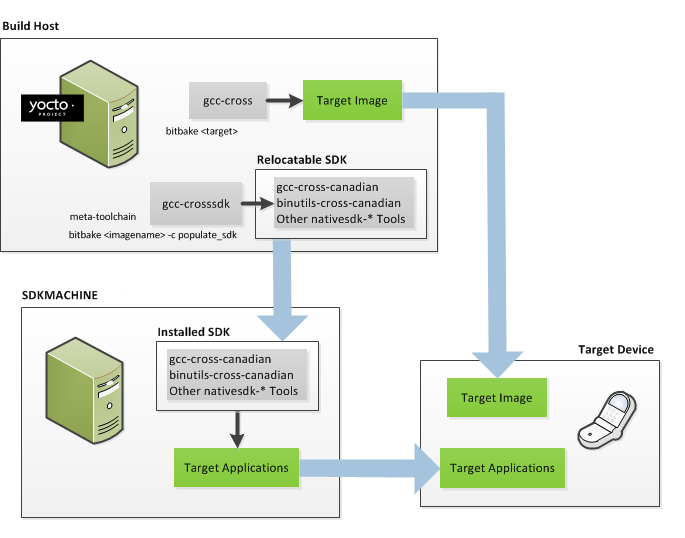
\includegraphics[scale=1]{cross-development-toolchains.png}
  \centering
  \caption{Toolchain di cross-sviluppo del progetto Yocto}
  \label{fig:ToolchainYocto}
\end{figure}

%% Interruzione di pagina
\newpage

\subsection{Framework OSGi}\label{OSGi}
In pausa finch\`e non sei sicuro di usarlo.

% Capitolo 3: Corpo della tesi. Sviluppo del progetto: cosa ho fatto e come l'ho fatto.
\chapter{Sviluppo del progetto}
In questo capitolo verr\`a riportato come \`e stato affrontato lo sviluppo dell'applicazione e come sono stati affrontati i problemi riscontrati.

\section{Analisi degli ambienti di sviluppo disponibili per l'image processing embedded}
Nella fase iniziale del progetto si \`e studiato quale potesse essere l'ambiente di sviluppo adatto all'applicazione. Sono state considerate principalmente due possibilit\`a analizzate nei paragrafi seguenti.

\subsection{Ambiente di sviluppo Xilinx}

\begin{table}[h!]
    \centering
	\begin{tabular}{|c|c|}
	\hline
	Hardware & Avnet Zedboard \\ \hline
	Acquisizione video & HDMI Webcam \\ \hline
    Ambiente di sviluppo & Xilinx SDSoC \\ \hline
    Piattaforma software & Bare-metal\\
    \hline
	\end{tabular}
    \caption{Riassunto componenti ambiente di sviluppo Xilinx}
\end{table}

Inizialmente si era pensato usare una scheda di sviluppo Xilinx che integrasse una CPU ARM e una FPGA, in modo che fosse possible sfruttare i tool di sintesi di alto livello messi a disposizione da Xilinx per lo sviluppo. Utilizzando questo ambiente di sviluppo integrato sarebbe stato possibile realizzare applicazioni ad altissime prestazioni con la flessibilit\`a di un linguaggio ad alto livello come C/C++. Uno dei target di punta di questi sistemi di sviluppo \`e appunto l'image processing e come supporto forniscono anche librerie proprietarie pre-ottimizzate per l'hardware Xilinx.

%% Interruzione di pagina
\newpage

\subsubsection{Hardware}
La piattaforma target sarebbe stata una Avnet Zedboard.

Specifiche tecniche:

\begin{table}[h!]
    \centering
	\begin{tabular}{|c|c|}
	\hline
    ZYNQ-7000 SOC XC7Z020 & Dual-core ARM Cortex-A9 + FPGA Kintex-7 \\ \hline
    Memoria & 512 MB DDR3 + 256 Mb Quad-SPI Flash + 4GB SD card \\ \hline
    Espansione & FMC (Low Pin Count) + Pmod headers (2x6) \\ \hline
    Video & HDMI output (1080p60 + audio) + VGA \\
    \hline
	\end{tabular}
    \caption{Specifiche tecniche Avnet Zedboard}
\end{table}

Purtroppo, avendo la scheda una sola porta HDMI disponibile solo in output \`e stato necessario procurarsi un modulo aggiuntivo da collegarsi all'header FMC per avere a disposizione anche una porta HDMI in ingresso.

In figura \ref{fig:Zynq7000} \`e riportato il diagramma del SoC Zynq-7000.

\begin{figure}[h!]
  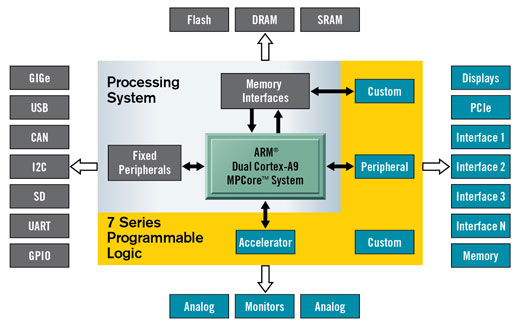
\includegraphics[width=\textwidth]{Zynq7000.jpg}
  \centering
  \caption{Diagramma del SoC Zynq-7000}
  \label{fig:Zynq7000}
\end{figure}

%% Interruzione di pagina
\newpage

\subsubsection{Piattaforma per lo sviluppo SDSoC}
La piattaforma per lo sviluppo SDSoC permette uno sviluppo integrato dell'applicativo e dell'IP hardware utilizzando un linguaggio di alto livello come il C o il C++. Vista la maggiore familiarit\`a con i linguaggi di alto livello l'utilizzo di questo ambiente di sviluppo avrebbe comportato una maggior flessibilit\`a e velocit\`a nello sviluppo con il vantaggio di potersi avvalere dell'accelerazione hardware sfruttando la FPGA presente sul SoC.

\begin{figure}[h!]
  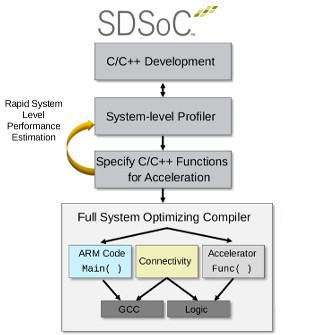
\includegraphics[scale=1]{XilinxSDSoC.png}
  \centering
  \caption{Workflow SDSoC}
  \label{fig:SDSoC}
\end{figure}

SDSoC permette di scrivere l'intera applicazione in codice di alto livello. In fase di compilazione si va a specificare quale funzione si vuole eseguire sulla FPGA, per sfruttarne l'accelerazione hardware. A seguito dell'intervento del programmatore per specificare mappatura della memoria e ottimizzazioni per l'esecuzione in hardware, \`e possibile eseguire l'applicazione sull'ARM Cortex ed eseguire le task pi\`u pesanti dal punto di vista computazionale sulla FPGA.

%% Interruzione di pagina
\newpage

\subsubsection{Compatibilit\`a con OpenCV e liberia AuvizCV}

\begin{figure}[h!]
  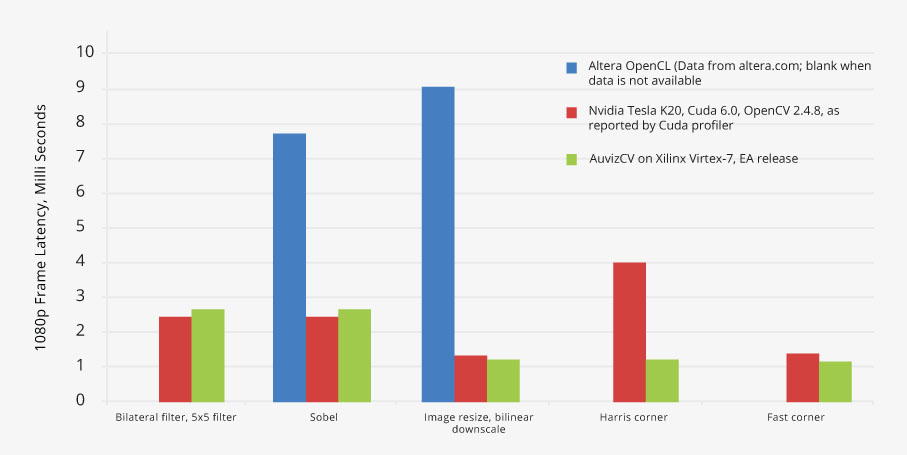
\includegraphics[width=\textwidth]{AuvizCV.jpg}
  \centering
  \caption{Risultati benchmark}
  \label{fig:BenchmarkAuvizCV}
\end{figure}

Come ulteriore punto a favore di questo ambiente, Xilinx vantava la compatibilit\`a del sistema con OpenCV per l'esecuzione su CPU mentre rendeva disponibile una libreria compatibile con OpenCV per l'esecuzione su FPGA. Quest'ultima prende il nome di \textbf{AuvizCV}, la quale non \`e altro che un subset delle funzioni disponibili in OpenCV pre-ottimizzate per l'esecuzione sulle FPGA Xilinx. Questa libreria sfrutta le potenzialit\`a di SDSoC in quanto \`e stata scritta interamente in codice di alto livello e, in fase di compilazione, le funzioni utilizzate vengono sintetizzate sulla FPGA. Questa API si mantiene coerente con OpenCV per facilitare l'implementazione e l'accelerazione in harware. In figura \ref{fig:BenchmarkAuvizCV} sono riportati i risultati dei benchmark confrontando l'accelerazione di alcuni algoritmi di OpenCV usando varie tecnologie.

%% Interruzione di pagina
\newpage

%TODO: Approfondire?
\subsection{Ambiente di sviluppo Intel - Yocto}

\begin{table}[h!]
    \centering
	\begin{tabular}{|c|c|}
	\hline
	Hardware & Eurotech ReliaGate 20-25 \\ \hline
	Acquisizione video & Webcam - Telecamere Intel RealSense \\ \hline
    Ambiente di sviluppo & Toolchain generata con Yocto \\ \hline
    Piattaforma software & Distribuzione Linux custom Poky \\
    \hline
	\end{tabular}
    \caption{Riassunto componenti ambiente di sviluppo Intel - Yocto}
\end{table}

Come seconda possibilit\`a si \`e considerata la possibilit\`a di usare l'hardware reso disponibile da Eurotech e realizzare da zero l'infrastruttura software sfruttando il progetto Yocto.

\subsubsection{Hardware}
L'azienda ha fornito come piattaforma hardware un ReliaGate 20-25 nonch\`e le telecamere Intel RealSense.

\begin{figure}[h!]
  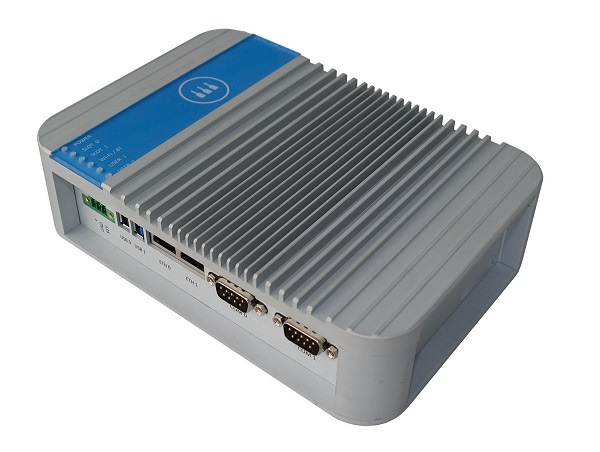
\includegraphics[scale=0.5]{ReliaGATE2025.jpg}
  \centering
  \caption{ReliaGate 20-25}
  \label{fig:ReliaGate2025}
\end{figure}

Specifiche tecniche:

\begin{table}[h!]
    \centering
	\begin{tabular}{|c|c|}
	\hline
    ReliaGate 20-25-33 & Processore Intel E3827 Dual Core 1.75GHz x86-64 \\ \hline
    Memoria & 2GB 1333MHz DDR3L ECC + 8GB eMMC \\ \hline
    Connettivit\`a & 1x USB 3.0 + 2x USB 2.0 + 2x RS-232/RS-422/RS-485 \\ \hline
    Video & mini DisplayPort \\
    \hline
	\end{tabular}
    \caption{Specifiche tecniche ReliaGate 20-25-33}
\end{table}

\subsubsection{Software e piattaforma per lo sviluppo}
Gli strumenti che si sarebbe andati ad utilizzare sono quelli di cui si \`e parlato nel capitolo 2. Yocto per la realizzazione della distribuzione Linux, la toolchain di Yocto per la cross-compilazione dei sorgenti, OpenCV per l'image processing e le telecamere RealSense con annessa libreria.

%% Interruzione di pagina
\newpage

\subsection{Motivazioni per la scelta finale}
Si � infine scelto di utilizzare l'ambiente di sviluppo Intel - Yocto per i seguenti motivi:
\begin{itemize}
\item Flessibilit\`a: la possibilit\`a di aggiungere librerie e strumenti software grazie al progetto Yocto permetteva di avere un ambiente di lavoro molto pi\`u flessibile della controparte Xilinx.
\item Completezza: la libreria AuvizCV, seppur molto performante, mancava di moltissime funzioni rispetto ad una installazione completa di OpenCV, la quale poteva essere comodamente installata sul ReliaGate.
\item Performance: la CPU Intel \`e molto pi\`u performante dell'ARM presente sulla Zedboard. Siccome sarebbe stato comunque necessario eseguire parte del codice OpenCV sulla CPU, si sarebbero perse molte performance usando l'ambiente Xilinx.
\item Compatibilit\`a: anche se inizialmente non era previsto l'impiego delle telecamere RealSense, la board Xilinx non sarebbe potuta essere compatibile con queste ultime vista la mancanza di una porta USB 3.0 e il supporto software.
\end{itemize}

Nei prossimi capitoli procederemo con la descrizione del codice che \`e stato realizzato per la realizzazione del Passenger Counter.

%% Interruzione di pagina
\newpage

\section{Passenger Counter con sottrazione del background}
In questa sezione tratteremo la prima versione realizzata del contatore di passeggeri. Questa prima versione non faceva uso delle telecamere RealSense e presentava alcune criticit\`a che vedremo nel seguito. 

Inizialmente, descriveremo l'hardware utilizzato, tratteremo le tecniche utilizzate, quindi passeremo a descrivere come sono state integrate nel codice ed il suo funzionamento. Infine parleremo dei risultati ottenuti da questa implementazione e le problematiche principali.

\subsection{Componenti hardware}
Per questa prima implementazione del contatore di passeggeri \`e stata utilizzata una semplice webcam.

\begin{table}[ht]
\begin{minipage}[b]{0.56\linewidth}
\centering
\begin{tabular}{ | c | c | }
    \hline
    Risoluzione & 640 x 480 \\ \hline
    Framerate & 30fps \\ \hline
	Connessione & USB 2.0 \\ \hline
    Tecnologia & driverless \\ \hline
    \end{tabular}
    \caption{Specifiche tecniche webcam}
    \label{table:SpecificheWebcam}
\end{minipage}\hfill
\begin{minipage}[b]{0.4\linewidth}
\centering
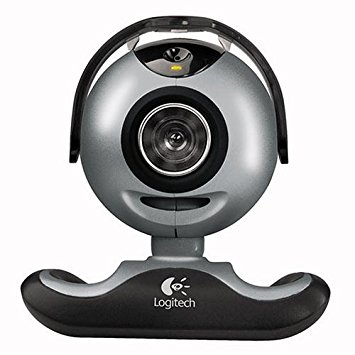
\includegraphics[width=40mm]{WebCam.jpg}
\captionof{figure}{Logitech QuickCam Pro 5000}
\label{fig:Webcam}
\end{minipage}
\end{table}

Essendo driverless veniva riconosciuta senza problemi dal ReliaGate ed \`e stato possibile leggere i frame in ingresso tramite OpenCV senza l'installazione di componenti software aggiuntivi.

% TODO: Approfondire? La matematica dietro il metodo \`e spiegata sufficientemente bene nella pagina di wikipedia
% link: 
\subsection{Algoritmo per la sottrazione del background}
La sottrazione del background \`e una tecnica, molto utilizzata dell'image processing e della computer vision, nella quale viene estratto il primo piano dell'immagine per essere ulteriormente manipolato. La background subtraction \`e una tecnica largamente utilizzata per rilevare soggetti in movimento all'interno di flussi video catturati da una telecamera statica.

L'algoritmo usato all'interno del codice di questa versione del contatore di passeggeri \`e basata su due paper pubblicati da Z.Zivkovic, "Improved adaptive Gausian mixture model for background subtraction" del 2004 e "Efficient Adaptive Density Estimation per Image Pixel for the Task of Background Subtraction" del 2006.

Questo algoritmo \`e anche noto come Gaussian Mixture-based Background/Foreground Segmentation Algorithm. Esso modella ogni pixel del background con una mixture di distribuzioni gaussiane selezionando automaticamente il numero appropriato da utilizzare. I pesi della mixture di gaussiane rappresentano il tempo per il quale quei colori permangono all'interno della scena. I colori che probabilmente appartengono al background sono quelli che rimangono per pi\`u tempo all'interno della scena e sono i pi\`u statici.

%% Interruzione di pagina
\newpage

Tipicamente, per facilitare l'elaborazione delle immagini a valle dell'applicazione dell'algoritmo di background subtraction, si ricava una immagine in scala di grigi nella quale i pixel neri rappresentano il background i pixel bianchi il primo piano. Nel caso dell'algoritmo usato per il Passenger Counter, le ombre vengono evidenziate con un colore grigio.
Qui di seguito \`e riportato un esempio di funzionamento.

\begin{figure}[h!]
  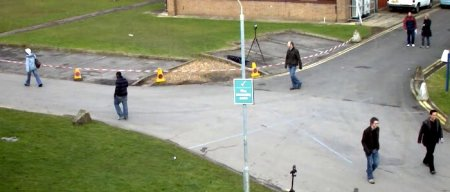
\includegraphics[width=.49\textwidth]{resframe.jpg}
  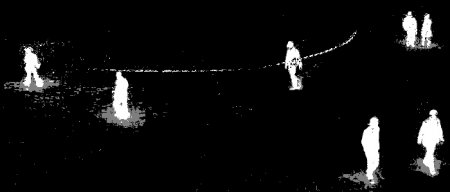
\includegraphics[width=.49\textwidth]{resmog2.jpg}
  \centering
  \caption{Esempio funzionamento BackgroundSubtractorMOG2}
  \label{fig:EsempioBackSub}
\end{figure}

Questo algoritmo \`e reso disponibile dalla libreria OpenCV per mezzo della funzione BackgroundSubtractorMOG2. Nel seguito vedremo come \`e stato utilizzato all'interno del codice del Passenger Counter.

% TODO: Chiedere al prof quanto approfondire che qua \`e un casino leggersi il paper
\subsection{Algoritmo per il rilevamento dei contorni}
L'algoritmo \`e descritto in Suzuki, S. and Abe, K., Topological Structural Analysis of Digitized Binary Images by Border Following. CVGIP 30 1, pp 32-46 (1985).

Questo algoritmo per la rilevazione dei contorni \`e utilizzato anche nella seconda versione del Passenger Counter.

Qui di seguito \`e riportato un esempio di funzionamento.

\begin{figure}[h!]
  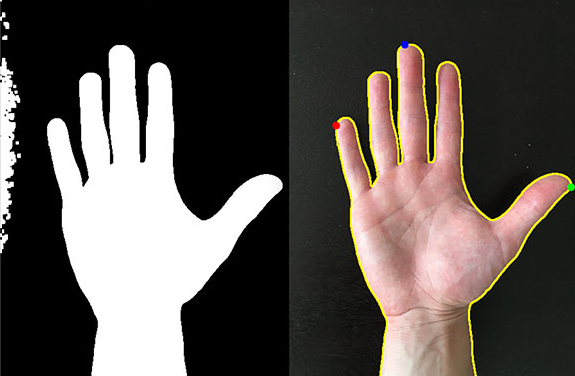
\includegraphics[scale=0.75]{findContours.png}
  \centering
  \caption{Esempio funzionamento findContours: l'immagine a sinistra rappresenta l'immagine di input in bianco e nero ricavata dall'immagine a colori. L'immagine a destra \`e stata ricavata disegnando i contorni ricavati per mezzo dell'algoritmo sull'immagine a colori.}
  \label{fig:EsempioFindContours}
\end{figure}

%% Interruzione di pagina
\newpage

\subsection{Titolo}
Suddivideremo il codice in tre sezioni principali:
\begin{enumerate}
\item Estrazione degli oggetti in movimento.
\item Rilevamento e tracking degli oggetti di nostro interesse.
\item Conteggio degli attraversamenti.
\end{enumerate}

\subsubsection{Estrazione degli oggetti in movimento}

\begin{lstlisting}[language=C++]
VideoCapture cap;

// Streams
Mat frame;       //input stream
Mat fgMaskMOG2;  //fg mask generated by MOG2 method
Mat morphTrans;  //fgMaskMOG2 after morphological transformations

Ptr<BackgroundSubtractor> pMOG2; //MOG2 Background subtractor

int history = 1000;
double varThreshold = BACKGROUN_SUB_THRESHOLD;
bool detectShadows = true;
pMOG2 = createBackgroundSubtractorMOG2(history, varThreshold, detectShadows);

while(!stop)
{
    // Wait for a frame from camera/video and store it into frame
    cap.read(frame);

    // --BACKGROUND SUBTRACTION
    pMOG2->apply(frame, fgMaskMOG2, 0.1);

    // --DENOISING
    // Threshold the image
    threshold(fgMaskMOG2, morphTrans, whiteThreshold, MAXRGBVAL, THRESH_BINARY);

    // Eroding
    erode(morphTrans,morphTrans, Mat(Size(erodeAmount,erodeAmount), CV_8UC1));

    // Dilating
    dilate(morphTrans,morphTrans, Mat(Size(dilateAmount,dilateAmount), CV_8UC1));

    // Blurring the image
    blur(morphTrans,morphTrans, Size(blur_ksize,blur_ksize));

    ...
}
\end{lstlisting}

%% Interruzione di pagina
\newpage

Il codice esegue le seguenti operazioni:
\begin{enumerate}
\item Anzitutto ci appoggiamo a OpenCV per andare a leggere i frame ricevuti dalla telecamera. Essi vengono direttamente convertiti in tipo Mat per poter essere manipolati facilmente da OpenCV.
\item I frame vengono passati alla funzione che applica la sottrazione del background. OpenCV prevede la creazione di un oggetto BackgroundSubtractor il quale ha tra i suoi metodi l'applicazione della sottrazione del background. Questo metodo produce come output una immagine in scala di grigi nella quale i pixel bianchi appartengono al primo piano, i pixel neri appartengono al background.
\item Seguono delle trasformazioni  sui frame necessarie a minimizzare il rumore nell'immagine e semplificare il lavoro della funzione di rilevazione dei contorni.
    \begin{enumerate}
    \item Threshold: viene applicata una soglia per eliminare le ombre. Ogni pixel il cui valore numerico \`e inferiore al valore dato come soglia (whiteThreshold) viene portato al valore MAXRGBVAL. Ogni pixel che si trova sotto la soglia viene posto a 0. Ovvero:
    
    \begin{equation}
    dstPixel(x,y) = \begin{cases} MAXRGBVAL, & \mbox{se } srcPixel(x,y) > threshold \\ 0, & \mbox{altrimenti } \end{cases}
    \end{equation}

    \item Erosione: Questa operazione ha come risultato quello di espandere le regioni scure dell'immagine. L'obiettivo \`e quello di eliminare il rumore bianco gaussiano dall'immagine.
    \item Dilatazione: Questa operazione ha come risultato quello di far "crescere" le regioni luminose dell'immagine. L'obiettivo \`e quello di rendere pi\`u facilmente rilevabili gli oggetti del primo piano.
    \item Blur: Questa operazione effettua una sfocatura dell'immagine. L'obiettivo \`e sempre quello di ridurre il rumore dell'immagine. Questa funzione utilizza una semplice filtro lineare.
    \end{enumerate}
\end{enumerate}

Risultato delle operazioni:

\begin{figure}[h!]
  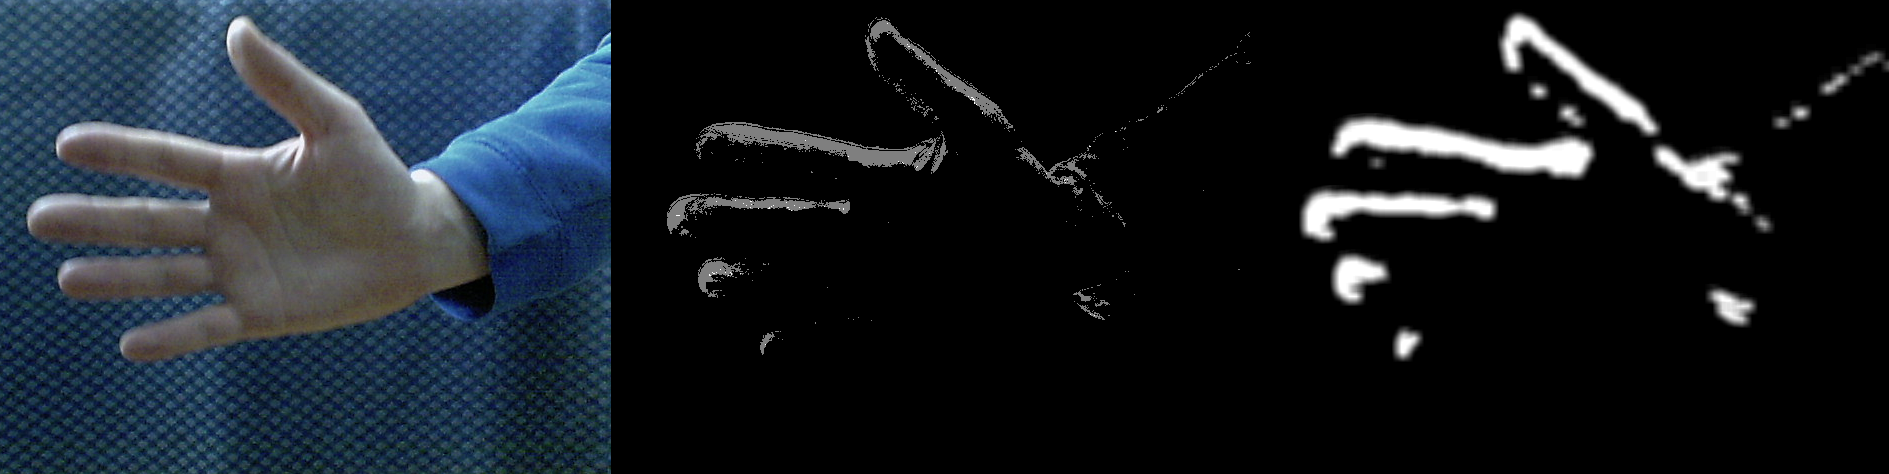
\includegraphics[width=\linewidth]{PCN1v2.png}
  \centering
  \caption{L'immagine a sinistra rappresenta l'input. L'immagine al centro \`e il risultato dell'applicazione della sottrazione del background. L'immagine a destra \`e l'output delle operazioni di sottrazione del rumore.}
  \label{fig:PCN1}
\end{figure}

%% Interruzione di pagina
\newpage

\subsubsection{Rilevamento e tracking degli oggetti di nostro interesse}

\begin{lstlisting}[language=C++]
while(!stop)
{
    ...

    // --FINDING CONTOURS
    findContours(morphTrans, contours, hierarchy, RETR_EXTERNAL, CHAIN_APPROX_NONE);

    // For every detected object
    for(unsigned int idx = 0; idx < contours.size(); idx++)
    {
        // -- AREA
        // Calculating area
        double areaCurrentObject = contourArea(contours[idx]);

        // If calculated area is big enough begin tracking the object
        if(areaCurrentObject > areaMin)
        {
            // Getting bounding rectangle
            Rect br = boundingRect(contours[idx]);
            Point2f mc = Point2f((int)(br.x + br.width/2) ,(int)(br.y + br.height/2) );

            // Drawing mass center and bounding rectangle
            rectangle( frame, br.tl(), br.br(), GREEN, 2, 8, 0 );
            circle( frame, mc, 5, RED, 2, 8, 0 );

            ...
        }

        ...
    }
}
\end{lstlisting}

%% Interruzione di pagina
\newpage
\subsubsection{Rilevamento e tracking degli oggetti di nostro interesse}

Il codice esegue le seguenti operazioni:

\begin{enumerate}
\item Ricava i contorni per mezzo della funzione di cui abbiamo discusso l'algoritmo nella sezione precedente.
\item Per ogni contorno completo rilevato dalla funzione eseguiamo le seguenti operazioni:
    \begin{enumerate}
    \item Ne calcoliamo l'area. Se supera una certa area minima, ricava sperimentalmente, decidiamo che si tratta di una persona.
    \item Ne ricaviamo il rettangolo che inscrive i controrni rilevati in precedenza tramite la funzione boundingRectangle.
    \item Di questo rettangolo rileviamo il centro.
    \item Per semplificare lo sviluppo e il debugging andiamo a disegnare questo rettangolo e questo centro sull'immagine a colori.
    \end{enumerate}
\end{enumerate}
L'informazione fondamentale per il resto dell'algoritmo \`e data dalla posizione del centro di questo rettangolo che rappresenter\`a la posizione dei passeggeri all'interno del raggio visivo della telecamera.

Risultato delle operazioni:

\begin{figure}[h!]
  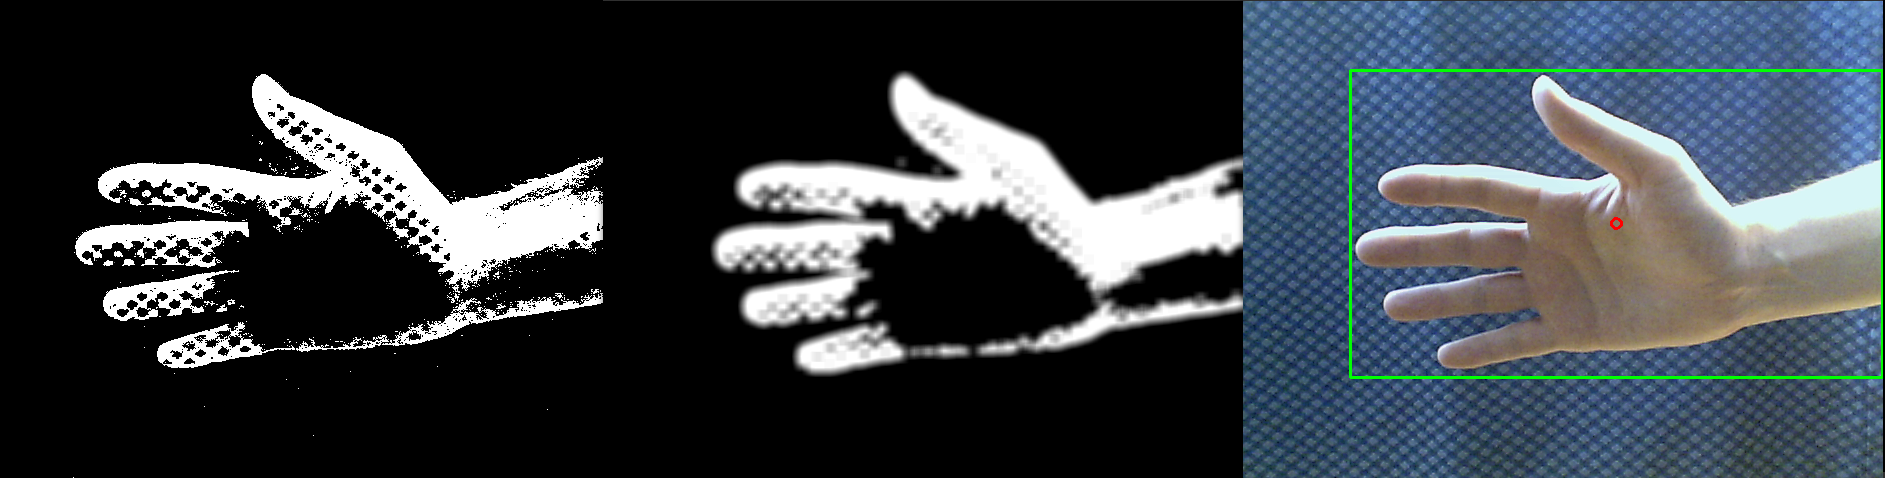
\includegraphics[width=\linewidth]{PCN2.png}
  \centering
  \caption{L'immagine a sinistra rappresenta l'immagine in ingresso dopo la sottrazione del background. L'immagine al centro \`e l'output delle operazioni di sottrazione del rumore. L'immagine a destra \`e l'immagine di ingresso sulla quale sono stati disegnati il bounding rectangle e il centro del rettangolo.}
  \label{fig:PCN2}
\end{figure}

%% Interruzione di pagina
\newpage

% TODO: Parlare della classe passengers e poi di come viene utilizzata
\subsubsection{Struttura per la rappresentazione delle entit\`a passeggeri}
Per il tracciamento dei passeggeri \`e stata creata una classe che contenesse le informazioni necessarie per il corretto tracking delle entit\`a.

\begin{lstlisting}[language=C++, caption=passenger.h]
class Passenger {

  public:

    // Constructor
    Passenger(int id, Point2f center, int newAge);

    // Selectors
    int getPid() {return pid;};

    Point2f getCenter() {return mc;};
    float getX(){return mc.x;};
    float getY(){return mc.y;};

    int getAge() {return age;};

    vector<Point> getTracks(){return tracks;};
    Scalar getTrackColor(){return trackColor;};

    Point getCurrentPoint(){return tracks[tracks.size()-1];};
    Point getLastPoint(){return tracks[tracks.size()-2];};

    // Methods
    void updateCoords(Point2f newCenter);
    void updateAge(){age++;return;};

  private:
    int pid;    // Passenger ID
    Point2f mc; // Mass center
    int age;    // Passenger age

    vector<Point> tracks;
    Scalar trackColor;

};
\end{lstlisting}

\begin{lstlisting}[language=C++, caption=passenger.cpp]
Passenger::Passenger(int id, Point2f center, int newAge = 0) {
    pid = id;
    mc = center;
    age = newAge;

    tracks.push_back(Point(center.x,center.y));
    trackColor = Scalar(rand() % 255, rand() % 255, rand() % 255);
}

void Passenger::updateCoords(Point2f newCenter) {
    mc = newCenter;

    tracks.push_back(Point(newCenter.x,newCenter.y));

    // If too many tracking points remove older points
    if(tracks.size() > MAX_TRACK_LENGTH) {
        tracks.erase(tracks.begin());
    }

    // Reset age
    // If the object is being tracked it means its active we don't want it to disappear
    age = 0;

    return;
}
\end{lstlisting}

Questa classe ha tre obiettivi principali:
\begin{enumerate}
\item Identificare univocamente le entit\`a che entrano nel raggio visivo della telecamera.
\item Memorizzare lo storico delle posizione occupate da tali entit\`a all'interno del raggio visivo della telecamera.
\item Tenere traccia del tempo per il quale l'entit\`a rimane all'intenro del raggio visivo della telecamera.
\end{enumerate}

Queste necessit\`a sono state assolte per mezzo delle seguenti variabili:
\begin{enumerate}
\item \textbf{pid}: \`e un intero assegnato in fase di registrazione all'entit\`a-passeggero. Esso andr\`a ad identificarlo univocamente all'interno del programma.
\item \textbf{tracks}: \`e un vettore di coordinate che conservano la posizione dei passeggeri. Il massimo numero di posizioni mantenute in memoria \`e stato deciso sperimentalmente.
\item \textbf{age}: \`e un intero che va a rappresentare da quanto tempo il passeggero non viene rilevato nel raggio d'azione della telecamera. Oltre un certo valore di questo parametro il passeggero verr\`a rimosso dalla memoria del contatore.
\end{enumerate}

Inolte \`e stata implementata anche la seguente variabile:
\begin{itemize}
\item trackColor: \`e un vettore di interi che vanno a rappresentare un colore RGB randomizzato. Viene usato per disegnare le tracce lasciate dal transito dei passeggeri nel raggio visivo della telecamera con colori diversi, in modo tale che sia facile verificare che il tracciamento sia avvenuto correttamente.
\end{itemize}

%% Interruzione di pagina
\newpage

\subsubsection{Conteggio degli attraversamenti}

%% Fine dei capitoli normali, inizio dei capitoli-appendice (opzionali)
\appendix

\part{Appendici}

\chapter{Altro capitolo}
Sed purus libero, vestibulum ut nibh vitae, mollis ultricies augue. Pellentesque velit libero, tempor sed pulvinar non, fermentum eu leo. Duis posuere eleifend nulla eget sagittis. Nam laoreet accumsan rutrum. Interdum et malesuada fames ac ante ipsum primis in faucibus. Curabitur eget libero quis leo porttitor vehicula eget nec odio. Proin euismod interdum ligula non ultricies. Maecenas sit amet accumsan sapien.

%% Parte conclusiva del documento; tipicamente per riassunto, bibliografia e/o indice analitico.
\backmatter

%% Riassunto (opzionale)
\summary
Maecenas tempor elit sed arcu commodo, dapibus sagittis leo egestas. Praesent at ultrices urna. Integer et nibh in augue mollis facilisis sit amet eget magna. Fusce at porttitor sapien. Phasellus imperdiet, felis et molestie vulputate, mauris sapien tincidunt justo, in lacinia velit nisi nec ipsum. Duis elementum pharetra lorem, ut pellentesque nulla congue et. Sed eu venenatis tellus, pharetra cursus felis. Sed et luctus nunc. Aenean commodo, neque a aliquam bibendum, mauris augue fringilla justo, et scelerisque odio mi sit amet diam. Nulla at placerat nibh, nec rutrum urna. Donec ut egestas magna. Aliquam erat volutpat. Phasellus vestibulum justo sed purus mattis, vitae lacinia magna viverra. Nulla rutrum diam dui, vel semper mi mattis ac. Vestibulum ante ipsum primis in faucibus orci luctus et ultrices posuere cubilia Curae; Donec id vestibulum lectus, eget tristique est.

%% Bibliografia (opzionale)
\bibliographystyle{plain_\languagename}%% Carica l'omonimo file .bst, dove \languagename � la lingua attiva.
%% Nel caso in cui si usi un file .bib (consigliato)
\bibliography{thud}
%% Nel caso di bibliografia manuale, usare l'environment thebibliography.

%% Per l'indice analitico, usare il pacchetto makeidx (o analogo).

\end{document}

--- Istruzioni per l'aggiunta di nuove lingue ---
Per ogni nuova lingua utilizzata aggiungere nel preambolo il seguente spezzone:
    \addto\captionsitalian{%
        \def\abstractname{Sommario}%
        \def\acknowledgementsname{Ringraziamenti}%
        \def\authorcontactsname{Contatti dell'autore}%
        \def\candidatename{Candidato}%
        \def\chairname{Direttore}%
        \def\conclusionsname{Conclusioni}%
        \def\cosupervisorname{Co-relatore}%
        \def\cosupervisorsname{Co-relatori}%
        \def\cyclename{Ciclo}%
        \def\datename{Anno accademico}%
        \def\indexname{Indice analitico}%
        \def\institutecontactsname{Contatti dell'Istituto}%
        \def\introductionname{Introduzione}%
        \def\prefacename{Prefazione}%
        \def\reviewername{Controrelatore}%
        \def\reviewersname{Controrelatori}%
        %% Anno accademico
        \def\shortdatename{A.A.}%
        \def\summaryname{Riassunto}%
        \def\supervisorname{Relatore}%
        \def\supervisorsname{Relatori}%
        \def\thesisname{Tesi di \expandafter\ifcase\csname thud@target\endcsname Laurea\or Laurea Magistrale\or Dottorato\fi}%
        \def\tutorname{Tutor aziendale%
        \def\tutorsname{Tutor aziendali}%
    }
sostituendo a "italian" (nella 1a riga) il nome della lingua e traducendo le varie voci.
